% Options for packages loaded elsewhere
% Options for packages loaded elsewhere
\PassOptionsToPackage{unicode}{hyperref}
\PassOptionsToPackage{hyphens}{url}
\PassOptionsToPackage{dvipsnames,svgnames,x11names}{xcolor}
%
\documentclass[
  brazilian,
  12pt,
  letterpaper,
  DIV=11,
  numbers=noendperiod]{scrartcl}
\usepackage{xcolor}
\usepackage[a4paper,left=3cm,right=2cm,top=3cm,bottom=2cm]{geometry}
\usepackage{amsmath,amssymb}
\setcounter{secnumdepth}{5}
\usepackage{iftex}
\ifPDFTeX
  \usepackage[T1]{fontenc}
  \usepackage[utf8]{inputenc}
  \usepackage{textcomp} % provide euro and other symbols
\else % if luatex or xetex
  \usepackage{unicode-math} % this also loads fontspec
  \defaultfontfeatures{Scale=MatchLowercase}
  \defaultfontfeatures[\rmfamily]{Ligatures=TeX,Scale=1}
\fi
\usepackage{lmodern}
\ifPDFTeX\else
  % xetex/luatex font selection
\fi
% Use upquote if available, for straight quotes in verbatim environments
\IfFileExists{upquote.sty}{\usepackage{upquote}}{}
\IfFileExists{microtype.sty}{% use microtype if available
  \usepackage[]{microtype}
  \UseMicrotypeSet[protrusion]{basicmath} % disable protrusion for tt fonts
}{}
\usepackage{setspace}
\makeatletter
\@ifundefined{KOMAClassName}{% if non-KOMA class
  \IfFileExists{parskip.sty}{%
    \usepackage{parskip}
  }{% else
    \setlength{\parindent}{0pt}
    \setlength{\parskip}{6pt plus 2pt minus 1pt}}
}{% if KOMA class
  \KOMAoptions{parskip=half}}
\makeatother
% Make \paragraph and \subparagraph free-standing
\makeatletter
\ifx\paragraph\undefined\else
  \let\oldparagraph\paragraph
  \renewcommand{\paragraph}{
    \@ifstar
      \xxxParagraphStar
      \xxxParagraphNoStar
  }
  \newcommand{\xxxParagraphStar}[1]{\oldparagraph*{#1}\mbox{}}
  \newcommand{\xxxParagraphNoStar}[1]{\oldparagraph{#1}\mbox{}}
\fi
\ifx\subparagraph\undefined\else
  \let\oldsubparagraph\subparagraph
  \renewcommand{\subparagraph}{
    \@ifstar
      \xxxSubParagraphStar
      \xxxSubParagraphNoStar
  }
  \newcommand{\xxxSubParagraphStar}[1]{\oldsubparagraph*{#1}\mbox{}}
  \newcommand{\xxxSubParagraphNoStar}[1]{\oldsubparagraph{#1}\mbox{}}
\fi
\makeatother


\usepackage{longtable,booktabs,array}
\newcounter{none} % for unnumbered tables
\usepackage{calc} % for calculating minipage widths
% Correct order of tables after \paragraph or \subparagraph
\usepackage{etoolbox}
\makeatletter
\patchcmd\longtable{\par}{\if@noskipsec\mbox{}\fi\par}{}{}
\makeatother
% Allow footnotes in longtable head/foot
\IfFileExists{footnotehyper.sty}{\usepackage{footnotehyper}}{\usepackage{footnote}}
\makesavenoteenv{longtable}
\usepackage{graphicx}
\makeatletter
\newsavebox\pandoc@box
\newcommand*\pandocbounded[1]{% scales image to fit in text height/width
  \sbox\pandoc@box{#1}%
  \Gscale@div\@tempa{\textheight}{\dimexpr\ht\pandoc@box+\dp\pandoc@box\relax}%
  \Gscale@div\@tempb{\linewidth}{\wd\pandoc@box}%
  \ifdim\@tempb\p@<\@tempa\p@\let\@tempa\@tempb\fi% select the smaller of both
  \ifdim\@tempa\p@<\p@\scalebox{\@tempa}{\usebox\pandoc@box}%
  \else\usebox{\pandoc@box}%
  \fi%
}
% Set default figure placement to htbp
\def\fps@figure{htbp}
\makeatother


% definitions for citeproc citations
\NewDocumentCommand\citeproctext{}{}
\NewDocumentCommand\citeproc{mm}{%
  \begingroup\def\citeproctext{#2}\cite{#1}\endgroup}
\makeatletter
 % allow citations to break across lines
 \let\@cite@ofmt\@firstofone
 % avoid brackets around text for \cite:
 \def\@biblabel#1{}
 \def\@cite#1#2{{#1\if@tempswa , #2\fi}}
\makeatother
\newlength{\cslhangindent}
\setlength{\cslhangindent}{1.5em}
\newlength{\csllabelwidth}
\setlength{\csllabelwidth}{3em}
\newenvironment{CSLReferences}[2] % #1 hanging-indent, #2 entry-spacing
 {\begin{list}{}{%
  \setlength{\itemindent}{0pt}
  \setlength{\leftmargin}{0pt}
  \setlength{\parsep}{0pt}
  % turn on hanging indent if param 1 is 1
  \ifodd #1
   \setlength{\leftmargin}{\cslhangindent}
   \setlength{\itemindent}{-1\cslhangindent}
  \fi
  % set entry spacing
  \setlength{\itemsep}{#2\baselineskip}}}
 {\end{list}}
\usepackage{calc}
\newcommand{\CSLBlock}[1]{\hfill\break\parbox[t]{\linewidth}{\strut\ignorespaces#1\strut}}
\newcommand{\CSLLeftMargin}[1]{\parbox[t]{\csllabelwidth}{\strut#1\strut}}
\newcommand{\CSLRightInline}[1]{\parbox[t]{\linewidth - \csllabelwidth}{\strut#1\strut}}
\newcommand{\CSLIndent}[1]{\hspace{\cslhangindent}#1}

\ifLuaTeX
\usepackage[bidi=basic,shorthands=off]{babel}
\else
\usepackage[bidi=default,shorthands=off]{babel}
\fi
\ifLuaTeX
  \usepackage{selnolig} % disable illegal ligatures
\fi


\setlength{\emergencystretch}{3em} % prevent overfull lines

\providecommand{\tightlist}{%
  \setlength{\itemsep}{0pt}\setlength{\parskip}{0pt}}



 


% Impede o sumário de colar na capa
\usepackage{tocloft}
\setcounter{tocdepth}{3}
\usepackage{placeins}
\usepackage{pdflscape}
\KOMAoption{captions}{tableheading}
\usepackage{xcolor}
\newcommand{\red}[1]{\textcolor{red}{#1}}
\newcommand{\blue}[1]{\textcolor{blue}{#1}}
\makeatletter
\@ifpackageloaded{caption}{}{\usepackage{caption}}
\AtBeginDocument{%
\ifdefined\contentsname
  \renewcommand*\contentsname{Índice}
\else
  \newcommand\contentsname{Índice}
\fi
\ifdefined\listfigurename
  \renewcommand*\listfigurename{Lista de Figuras}
\else
  \newcommand\listfigurename{Lista de Figuras}
\fi
\ifdefined\listtablename
  \renewcommand*\listtablename{Lista de Tabelas}
\else
  \newcommand\listtablename{Lista de Tabelas}
\fi
\ifdefined\figurename
  \renewcommand*\figurename{Figura}
\else
  \newcommand\figurename{Figura}
\fi
\ifdefined\tablename
  \renewcommand*\tablename{Tabela}
\else
  \newcommand\tablename{Tabela}
\fi
}
\@ifpackageloaded{float}{}{\usepackage{float}}
\floatstyle{ruled}
\@ifundefined{c@chapter}{\newfloat{codelisting}{h}{lop}}{\newfloat{codelisting}{h}{lop}[chapter]}
\floatname{codelisting}{Listagem}
\newcommand*\listoflistings{\listof{codelisting}{Lista de Listagens}}
\makeatother
\makeatletter
\makeatother
\makeatletter
\@ifpackageloaded{caption}{}{\usepackage{caption}}
\@ifpackageloaded{subcaption}{}{\usepackage{subcaption}}
\makeatother
\usepackage{bookmark}
\IfFileExists{xurl.sty}{\usepackage{xurl}}{} % add URL line breaks if available
\urlstyle{same}
\hypersetup{
  pdflang={pt-BR},
  colorlinks=true,
  linkcolor={blue},
  filecolor={Maroon},
  citecolor={Blue},
  urlcolor={Blue},
  pdfcreator={LaTeX via pandoc}}


\author{}
\date{}
\begin{document}


\setstretch{1.5}
\begin{titlepage}
\centering

% --- IMAGEM NO TOPO ---

\includegraphics[width=0.3\textwidth]{figuras/logo_ufmg.jpg}

{\large UNIVERSIDADE FEDERAL DE MINAS GERAIS \par}
{\large Instituto de Ciências Exatas \par}
{\large Departamento de Ciência da Computação e Estatística \par}
{\large Pós-Graduação Lato Sensu em Ciência de Dados \par}

\vspace{2cm}

{\bfseries\Large Uma Análise Comparativa entre Inferência Frequentista e Bayesiana em Modelos de Regressão Binária Aplicada a Risco de Crédito \par}

\vspace{2cm}

{\large Ana Beatriz Coelho Rodrigues \par}

\vfill

{\large Belo Horizonte \par}


{\large Ago/2026 \par}

\end{titlepage}

\newpage
\begin{center}

Ana Beatriz Coelho Rodrigues

\vspace{1cm}

{\bfseries\Large Uma Análise Comparativa entre Inferência Frequentista e Bayesiana em Modelos de Regressão Binária Aplicada a Risco de Crédito}


\vspace{2cm}

\begin{flushright}
Monografia apresentada ao Curso de Especialização em Ciência de Dados com Ênfase em Estatística da Universidade Federal de Minas Gerais como requisito parcial para obtenção do grau de Especialista em Ciência de Dados.


\vspace{1cm}

Orientador(a): Prof.(a) Dr.(a) Fábio N. Demarqui~
\end{flushright}

\vfill

Belo Horizonte  

Ago/2026
\end{center}
\newpage

\newpage
\begin{center}
{\bfseries\Large RESUMO}
\end{center}

\vspace{1cm}

\textcolor{red}{reavaliar os resumos, quando o trabalho estiver concluído}

Este trabalho tem como objetivo comparar as abordagens de inferência frequentista e bayesiana no contexto de modelos de classificação. O foco principal do estudo está na análise das diferenças conceituais, inferenciais e preditivas entre essas duas abordagens estatísticas, utilizando um conjunto de dados reais como estudo de caso para a aplicação dos modelos.

Inicialmente, são discutidos os fundamentos teóricos das abordagens frequentista e bayesiana, destacando suas principais características, pressupostos e formas de interpretação dos parâmetros. Em seguida, realiza-se uma análise exploratória dos dados com o objetivo de compreender a estrutura das variáveis e subsidiar a construção dos modelos, sem que a análise dos dados constitua o foco central do trabalho.

Na etapa de modelagem, são ajustados modelos de classificação sob as perspectivas frequentista e bayesiana, permitindo a comparação entre as abordagens quanto ao desempenho preditivo, à interpretação dos coeficientes estimados e à quantificação da incerteza associada às estimativas. A avaliação dos modelos é realizada por meio de métricas adequadas de classificação, possibilitando uma análise sistemática das diferenças e semelhanças entre os métodos.

Por fim, os resultados obtidos evidenciam as vantagens e limitações de cada abordagem no contexto de problemas de classificação binária, contribuindo para uma compreensão mais aprofundada das implicações práticas e metodológicas da escolha entre inferência frequentista e bayesiana em aplicações de análise de risco de crédito e ciência de dados.

\vspace{1cm}

\noindent\textbf{Palavras-chave:} regressão estatística; inferência frequentista; inferência bayesiana; modelos preditivos; análise de risco de crédito.
\newpage

\newpage
\begin{center}
{\bfseries\Large ABSTRACT}
\end{center}

\vspace{1cm}

This study aims to compare frequentist and Bayesian inference approaches in the context of regression models applied to the prediction of loan approval decisions. 

\vspace{1cm}

\noindent\textbf{Keywords:} frequentist inference; Bayesian inference; regression models; predictive modeling; credit risk analysis.
\newpage

\tableofcontents
\newpage

\textbf{Legenda de status do documento}

\begin{itemize}
\tightlist
\item
  \textbf{{[}TBD{]}} → tópico ainda indefinido; estrutura ou escopo em
  discussão
\item
  \textbf{{[}TO DO{]}} → tópico planejado, ainda não iniciado
\item
  \textbf{{[}WIP{]}} → em desenvolvimento
\item
  \textbf{{[}DRAFT{]}} → versão preliminar do texto
\item
  \textbf{{[}CHECK{]}} → verificação pendente (conceitos, dados, código
  ou referências)
\item
  \textbf{{[}REVISÃO{]}} → versão completa, pronta para avaliação

  \begin{itemize}
  \tightlist
  \item
    \textbf{{[}REVISÃO-1{]}} → para uma primeira versão
  \end{itemize}
\item
  \textbf{{[}AJUSTAR{]}} → ajustes finos de redação, figuras ou
  formatação (após revisão)
\item
  \textbf{{[}FINAL{]}} → versão definitiva (após revisão e ajustes
  finais)
\end{itemize}

\red{dúvidas, pendências, decisões em aberto}
\blue{comentários editoriais e lembretes}

\section{{[}TBD{]} Introdução}\label{tbd-introduuxe7uxe3o}

\begin{itemize}
\tightlist
\item
  Contexto de risco de crédito (motivação do trabalho)
\item
  Importância de modelos estatísticos na decisão financeira (com
  referencias de estudos anteriores)
\item
  Diferença conceitual entre abordagem frequentista e bayesiana
\item
  Motivação do estudo
\item
  Objetivo geral (resumida)
\item
  indicar as técnicas Estatísticas/Computacionais que serão utilizadas
  para a resolução do problema.
\item
  Estrutura do trabalho (Este trabalho está assim organizado: Na Seção 2
  apresentamos\ldots. A Seção 3 trata de\ldots{} )
\end{itemize}

\section{{[}TO DO{]} Referencial
Teórico}\label{to-do-referencial-teuxf3rico}

\blue{um dos principais capítulos, já que o foco do trabalho é a comparação entre abordagens.}

\subsection{{[}TO DO{]} Fundamentos de Probabilidade e Inferência
Estatística}\label{to-do-fundamentos-de-probabilidade-e-inferuxeancia-estatuxedstica}

\subsubsection{{[}TO DO{]} Variáveis Aleatórias e Distribuições de
Probabilidade}\label{to-do-variuxe1veis-aleatuxf3rias-e-distribuiuxe7uxf5es-de-probabilidade}

A formalização da incerteza em experimentos aleatórios ocorre por meio
de variáveis aleatórias, que representam os resultados de um espaço
amostral em uma escala numérica. Essa estrutura fundamenta o tratamento
quantitativo de dados e a construção de modelos de probabilidade,
servindo de base tanto para a inferência frequentista quanto para a
abordagem bayesiana.

As variáveis aleatórias são classificadas em discretas ou contínuas, a
depender da natureza de seu suporte. As discretas assumem valores em
conjuntos finitos ou enumeráveis, como a decisão de aprovação de crédito
ou o número de ocorrências de inadimplência. Já as contínuas podem
assumir qualquer valor em intervalos reais, como a renda dos proponentes
ou o tempo até o default. A incerteza inerente a essas variáveis é
formalizada por distribuições de probabilidade: no domínio discreto,
pela função de massa de probabilidade e, no contínuo, pela função
densidade de probabilidade. Tais funções não apenas sintetizam a
natureza probabilística das variáveis, mas viabilizam o cálculo de
medidas fundamentais, como esperança, variância e probabilidades
condicionais, elementos centrais para a modelagem de risco. A escolha
apropriada de distribuições de probabilidade é fundamental para capturar
a variabilidade dos dados observados e para a construção de modelos
inferenciais capazes de quantificar a incerteza associada às previsões.

\subsubsection{{[}TO DO{]} Inferência
Estatística}\label{to-do-inferuxeancia-estatuxedstica}

A inferência estatística reúne os métodos que permitem extrair
conclusões sobre uma população ampla a partir de uma amostra reduzida.
Na prática, quando não é viável analisar cada indivíduo ou produto de um
grupo inteiro, utilizamos os dados amostrais para realizar estimativas e
previsões, fundamentadas em modelos que conectam o que observamos aos
parâmetros que desejamos descobrir.

O elemento central desse processo é a aceitação da incerteza. Como os
dados estão sujeitos a variações e erros de medição, a inferência
utiliza estruturas probabilísticas para descrever o comportamento da
população (o conjunto total de elementos) com base na amostra, que é o
subconjunto efetivamente analisado. Como a população é quase sempre
muito maior que a amostra, as conclusões obtidas não são certezas
absolutas, mas sim afirmações probabilísticas. O processo consiste em
utilizar uma amostra aleatória para testar o modelo estatístico que
representa a população, acompanhando cada conclusão de uma medida que
quantifica o seu grau de confiabilidade. Esse caminho envolve escolher
um modelo adequado para o fenômeno e deduzir informações sobre seus
parâmetros desconhecidos.

\subsubsection{{[}TO DO{]} Interpretações da
probabilidade}\label{to-do-interpretauxe7uxf5es-da-probabilidade}

A noção de probabilidade ocupa um papel central na inferência
estatística, sendo a base para quantificar e interpretar a incerteza.
Atualmente, essa análise é conduzida por dois grandes paradigmas, o
frequentista e o bayesiano, que se distinguem essencialmente na
interpretação do conceito de probabilidade e no tratamento da incerteza
dos parâmetros.

Na abordagem frequentista, também chamada de clássica, a probabilidade é
entendida a partir da repetição de um experimento sob as mesmas
condições. Dentro dessa visão, a probabilidade é vista como uma
característica objetiva do processo que gera os dados, e não como algo
que depende do observador. Os dados coletados são tratados como
realizações aleatórias, enquanto os parâmetros do modelo estatístico que
descreve a população são considerados valores fixos, ainda que
desconhecidos. Assim, a incorporação de novas observações não altera
diretamente o conceito de probabilidade, mas contribui para estimativas
mais precisas desses parâmetros por meio de métodos inferenciais.

Já na abordagem bayesiana, a probabilidade assume um papel mais amplo.
Ela passa a representar o grau de confiança em uma afirmação, levando em
conta as informações disponíveis. Nesse contexto, a probabilidade pode
ser atribuída não apenas a eventos observáveis, mas também a hipóteses e
parâmetros do modelo. Os parâmetros populacionais desconhecidos são
tratados como variáveis aleatórias, cuja incerteza é descrita por
distribuições de probabilidade. Além disso, é possível incorporar
conhecimento prévio ao processo inferencial por meio de distribuições a
priori. À medida que novos dados são observados, esse conhecimento é
atualizado de forma sistemática pelo teorema de Bayes, resultando em uma
distribuição a posteriori que reflete tanto as informações anteriores
quanto a evidência empírica fornecida pelos dados.

\begin{itemize}
\tightlist
\item
  Probabilidade frequentista Definição como limite de frequências
  relativas Parâmetros como valores fixos desconhecidos Dados como
  realizadores aleatórios
\item
  Probabilidade como grau de crença (bayesiana) Probabilidade como
  medida de incerteza subjetiva/coerente Parâmetros como variáveis
  aleatórias
\end{itemize}

\subsubsection{{[}TO DO{]} Teorema de
Bayes}\label{to-do-teorema-de-bayes}

Teorema como mecanismo de atualização de crenças Relação entre: priori
verossimilhança posteriori Interpretação inferencial, não só matemática

\subsection{{[}TO DO{]} Problemas de Classificação em Aprendizado
Estatístico}\label{to-do-problemas-de-classificauxe7uxe3o-em-aprendizado-estatuxedstico}

\subsubsection{{[}TO DO{]} Classificação binária e
probabilistica}\label{to-do-classificauxe7uxe3o-binuxe1ria-e-probabilistica}

\subsubsection{{[}TO DO{]} Função de perda e
decisão}\label{to-do-funuxe7uxe3o-de-perda-e-decisuxe3o}

\begin{itemize}
\tightlist
\item
  Separabilidade linear e não linear \#\#\# {[}TO DO{]} Overfitting e
  generalização e Trade off viés-variancia (preparando terreno para
  problemas de crédito, onde a separação perfeita é improvável e o
  trade-off entre viés e variância é crucial) \#\#\# {[}TO DO{]}
  Probabilidades preditas vs.~classes previstas e Threshold de decisão e
  custo de erro
\end{itemize}

\subsection{{[}TO DO{]} Avaliação de Modelos de
Classificação}\label{to-do-avaliauxe7uxe3o-de-modelos-de-classificauxe7uxe3o}

\begin{itemize}
\tightlist
\item
  Desbalanceamento de classes (muito comum em dados de crédito, mas não
  no dataset atual) \#\#\# {[}TO DO{]} Matriz de confusão
\item
  Accuracy, Precision, Recall, F1-score
\item
  Custo assimétrico de erros (FP vs FN) \#\#\# {[}TO DO{]} Curvas
\item
  Curvas Precision--Recall
\item
  Curva ROC e AUC
\item
  Trade-off entre sensibilidade e especificidade
\end{itemize}

\subsection{{[}TO DO{]} Regressão Logística
Frequentista}\label{to-do-regressuxe3o-loguxedstica-frequentista}

\subsubsection{{[}TO DO{]} Formulação do
modelo}\label{to-do-formulauxe7uxe3o-do-modelo}

\begin{itemize}
\tightlist
\item
  Assumptions do modelo (e.g., independência, linearidade no logit,
  ausência de multicolinearidade)
\item
  Parametrização e interpretação
\item
  Interpretação dos coeficientes
\item
  Função logística \#\#\# {[}TO DO{]} Estimação por máxima
  verossimilhança (e a função de verossimilhança) A função de
  verossimilhança é comum na abordagem frequentista e Bayesiana
\item
  Testes de hipótese
\item
  Intervalos de confiança
\item
  Limitações da abordagem frequentista
\end{itemize}

\subsubsection{{[}TO DO{]} Interpretação dos
coeficientes}\label{to-do-interpretauxe7uxe3o-dos-coeficientes}

\begin{itemize}
\tightlist
\item
  Odds e odds ratio
\end{itemize}

\subsubsection{{[}TO DO{]} Diagnóstico e qualidade do
ajuste}\label{to-do-diagnuxf3stico-e-qualidade-do-ajuste}

\begin{itemize}
\tightlist
\item
  Análise de Resíduos
\item
  Análise de Multicolinearidade
\item
  Fisher Scoring
\end{itemize}

\subsubsection{{[}TO DO{]}}\label{to-do}

\subsection{{[}TO DO{]} Inferência
Bayesiana}\label{to-do-inferuxeancia-bayesiana}

\subsubsection{{[}TO DO{]} Priori}\label{to-do-priori}

\subsubsection{{[}TO DO{]} Posteriori}\label{to-do-posteriori}

\subsubsection{{[}TO DO{]} Atualização bayesiana e
incerteza}\label{to-do-atualizauxe7uxe3o-bayesiana-e-incerteza}

\begin{itemize}
\tightlist
\item
  Teorema de Bayes aplicado à estatística
\item
  diferenças conceituais
\item
  parametros como variáveis aleatórias
\item
  Priors, likelihood e posterior
\item
  Incerteza e distribuição posterior
\item
  Vantagens da abordagem bayesiana
\item
  Atualização sequencial da evidência
\item
  Interpretação probabilística
\item
  controle de sobreajuste (\ldots)
\end{itemize}

\subsection{{[}TO DO{]} Regressão Logística
Bayesiana}\label{to-do-regressuxe3o-loguxedstica-bayesiana}

\blue{(sempre traçando paralelos com a versão frequentista, principalmente os tópicos)}

\subsubsection{{[}TO DO{]} Formulação do
modelo}\label{to-do-formulauxe7uxe3o-do-modelo-1}

\begin{itemize}
\tightlist
\item
  Formulação do modelo probabilístico \#\#\# {[}TO DO{]} Escolha de
  priors \#\#\# {[}TO DO{]} Inferência
\item
  via MCMC \#\#\# {[}TO DO{]} Diagnóstico de convergência
\item
  (R-hat, traceplots)
\item
  Intervalos de credibilidade
\item
  Sensibilidade a priors
\item
  Robustez em pequenas amostras
\item
  Interpretação dos coeficientes sob posterior
\item
  Comparação direta de MLE- maximum likelyhood estimation e MAP-
  Maximum-a-Posteriori
\end{itemize}

(\ldots)

\subsection{{[}TO DO{]} Aplicações em Risco de Crédito e
Finanças/Saude}\label{to-do-aplicauxe7uxf5es-em-risco-de-cruxe9dito-e-finanuxe7assaude}

\blue{Não estender muito, acho que 1 página já deve ser suficiente}

(Contextualização)

\begin{itemize}
\item
  Modelos de scoring de crédito
\item
  Variáveis financeiras e risco
\item
  Decisão de concessão de empréstimos
\item
  Uso das probabilidades preditas para gestão de risco
\item
  Transparência e interpretabilidade
\item
  Em problemas de concessão de empréstimos, a incerteza é tão importante
  quanto a previsão.
\item
  O enfoque bayesiano permite incorporar conhecimento prévio do risco.
\item
  O enfoque frequentista fornece base tradicional de modelos de scoring.
\item
  A comparação entre ambas abordagens permite avaliar robustez das
  decisões.
\end{itemize}

\section{{[}WIP{]} Metodologia}\label{wip-metodologia}

\subsection{{[}REVISÃO-1{]} Descrição dos
Dados}\label{revisuxe3o-1-descriuxe7uxe3o-dos-dados}

\subsubsection{Descrição: Loan Approval
Dataset}\label{descriuxe7uxe3o-loan-approval-dataset}

Os modelos desenvolvidos neste trabalho utilizam dois conjuntos de dados
públicos. O primeiro conjunto de dados é o Loan Approval Dataset,
disponibilizado na plataforma Kaggle (Grewal (2026)), que contém
informações socioeconômicas e de crédito de clientes solicitando
empréstimos. A variável resposta é binária, indicando se o empréstimo
foi aprovado ou rejeitado. A Tabela~\ref{tbl-descricao-emprestimos}
apresenta uma descrição detalhada de todas as variáveis preditoras
incluídas no conjunto de dados.

\begin{longtable}[]{@{}ll@{}}
\caption{Descrição das variáveis do dataset de
emprestimos}\label{tbl-descricao-emprestimos}\tabularnewline
\toprule\noalign{}
Feature & Descrição \\
\midrule\noalign{}
\endfirsthead
\toprule\noalign{}
Feature & Descrição \\
\midrule\noalign{}
\endhead
\bottomrule\noalign{}
\endlastfoot
num\_dependentes & Número de dependentes do solicitante \\
escolaridade & Nível de escolaridade (Graduate / Not Graduate) \\
autonomo & Autônomo (Yes / No) \\
renda\_anual & Renda anual \\
valor\_emprestimo & Valor do empréstimo \\
prazo\_anos & Prazo em anos \\
score\_credito & Score de crédito \\
ativos\_residenciais & Bens residenciais, em valor monetário \\
ativos\_comerciais & Bens comerciais, em valor monetário \\
ativos\_luxo & Bens de luxo, em valor monetário \\
ativos\_bancarios & Ativos bancários, em valor monetário \\
status & Variável alvo (Approved = 1/Rejected = 0) \\
\end{longtable}

Por se tratar de um dataset estruturado especificamente para fins de
aprendizado de máquina e análise estatística, ele oferece um cenário
controlado, permitindo focar na sensibilidade dos modelos aos preditores
e na quantificação da incerteza sem as inconsistências típicas de bases
de dados administrativas brutas.

\subsubsection{Descrição: Dataset de Inadimplência de Cartões de
Crédito}\label{descriuxe7uxe3o-dataset-de-inadimpluxeancia-de-cartuxf5es-de-cruxe9dito}

Como segundo conjunto de dados, este trabalho também utiliza o
\texttt{Default\ of\ Credit\ Card\ Clients\ Dataset}, originalmente
disponibilizado por Yeh e Lien (Yeh; Lien (2009)) e atualmente mantido
no UCI Machine Learning Repository (Lichman (2013)). O conjunto reúne
informações de clientes de cartão de crédito em Taiwan, abrangendo o
período de abril a setembro de 2005, incluindo variáveis demográficas,
dados financeiros, histórico de pagamentos e valores de fatura. A
variável alvo é binária, denotada por \texttt{PD30} (Probability of
Default in 30 days), a qual indica a ocorrência de inadimplência no
horizonte de 30 dias --- operacionalmente definida, neste conjunto de
dados, como a inadimplência observada no mês subsequente. Assim, embora
\texttt{PD30} seja um conceito probabilístico no contexto de risco de
crédito, neste estudo ela é observada como uma variável indicadora,
assumindo valor 1 quando ocorre inadimplência e 0 caso contrário.

A inclusão deste segundo conjunto de dados tem dois objetivos
principais: (i) avaliar a capacidade de generalização dos modelos
desenvolvidos em um domínio distinto de crédito, e (ii) comparar o
desempenho preditivo e a interpretabilidade de diferentes abordagens de
modelagem e estratégias de seleção de variáveis. A
Tabela~\ref{tbl-descricao-inadimplencia} apresenta uma descrição
detalhada das variáveis presentes neste conjunto de dados, incluindo
informações demográficas, financeiras e comportamentais dos clientes.

\begin{longtable}[]{@{}
  >{\raggedright\arraybackslash}p{(\linewidth - 2\tabcolsep) * \real{0.4211}}
  >{\raggedright\arraybackslash}p{(\linewidth - 2\tabcolsep) * \real{0.5789}}@{}}
\caption{Descrição das variáveis do dataset de
inadimplência}\label{tbl-descricao-inadimplencia}\tabularnewline
\toprule\noalign{}
\begin{minipage}[b]{\linewidth}\raggedright
Feature
\end{minipage} & \begin{minipage}[b]{\linewidth}\raggedright
Descrição
\end{minipage} \\
\midrule\noalign{}
\endfirsthead
\toprule\noalign{}
\begin{minipage}[b]{\linewidth}\raggedright
Feature
\end{minipage} & \begin{minipage}[b]{\linewidth}\raggedright
Descrição
\end{minipage} \\
\midrule\noalign{}
\endhead
\bottomrule\noalign{}
\endlastfoot
\texttt{id\_cliente} & Identificador único de cada cliente \\
\texttt{limite\_credito} & Limite de crédito concedido ao cliente
(inclui crédito individual e suplementar) \\
\texttt{sexo} & Sexo do cliente (1 = masculino, 2 = feminino) \\
\texttt{escolaridade} & Nível de escolaridade (1 = pós-graduação, 2 =
universidade, 3 = ensino médio, 4 = outros) \\
\texttt{estado\_civil} & Estado civil (1 = casado, 2 = solteiro, 3 =
outros) \\
\texttt{idade} & Idade do cliente, em anos \\
\texttt{atraso\_pagto\_0} & Status de atraso no pagamento no mês
09/2005 \\
\texttt{atraso\_pagto\_2} & Status de atraso no pagamento no mês
08/2005 \\
\texttt{atraso\_pagto\_3} & Status de atraso no pagamento no mês
07/2005 \\
\texttt{atraso\_pagto\_4} & Status de atraso no pagamento no mês
06/2005 \\
\texttt{atraso\_pagto\_5} & Status de atraso no pagamento no mês
05/2005 \\
\texttt{atraso\_pagto\_6} & Status de atraso no pagamento no mês
04/2005 \\
\texttt{fatura\_valor\_1} & Valor da fatura no mês 09/2005 (NT
dollar) \\
\texttt{fatura\_valor\_2} & Valor da fatura no mês 08/2005 (NT
dollar) \\
\texttt{fatura\_valor\_3} & Valor da fatura no mês 07/2005 (NT
dollar) \\
\texttt{fatura\_valor\_4} & Valor da fatura no mês 06/2005 (NT
dollar) \\
\texttt{fatura\_valor\_5} & Valor da fatura no mês 05/2005 (NT
dollar) \\
\texttt{fatura\_valor\_6} & Valor da fatura no mês 04/2005 (NT
dollar) \\
\texttt{pagto\_valor\_1} & Valor pago no mês 09/2005 (NT dollar) \\
\texttt{pagto\_valor\_2} & Valor pago no mês 08/2005 (NT dollar) \\
\texttt{pagto\_valor\_3} & Valor pago no mês 07/2005 (NT dollar) \\
\texttt{pagto\_valor\_4} & Valor pago no mês 06/2005 (NT dollar) \\
\texttt{pagto\_valor\_5} & Valor pago no mês 05/2005 (NT dollar) \\
\texttt{pagto\_valor\_6} & Valor pago no mês 04/2005 (NT dollar) \\
\texttt{PD30} & Indicador binário de inadimplência no mês seguinte (1 =
sim, 0 = não) \\
\end{longtable}

\subsection{{[}TBD{]} Análise
Exploratória}\label{tbd-anuxe1lise-exploratuxf3ria}

\red{Apenas se tivermos tempo}

\subsection{{[}REVISÃO-1{]}
Pré-processamento}\label{revisuxe3o-1-pruxe9-processamento}

\subsubsection{{[}REVISÃO-1{]} Estrutura de dados e tratamento de
valores
ausentes}\label{revisuxe3o-1-estrutura-de-dados-e-tratamento-de-valores-ausentes}

Inicialmente, foi realizada a inspeção da estrutura do banco de dados,
com o objetivo de confirmar a consistência dos tipos das variáveis e a
adequação do formato dos dados às técnicas de modelagem adotadas. Essa
análise compreendeu a identificação das classes das variáveis, a
distinção entre atributos numéricos e categóricos e a validação da
variável resposta quanto à sua natureza e domínio.

Por fim, a presença de valores ausentes foi avaliada por meio da função
\texttt{is.na()}, com sumarização via \texttt{colSums(is.na())}. Não
foram identificadas observações faltantes no conjunto de dados,
eliminando a necessidade de técnicas de imputação e evitando a
introdução de incerteza adicional ou viés sistemático no processo de
estimação.

\subsubsection{{[}REVISÃO-1{]} Outliers}\label{revisuxe3o-1-outliers}

A identificação de valores atípicos (\emph{outliers}) nas variáveis
numéricas foi realizada por meio do critério do intervalo interquartil
(\emph{Interquartile Range}, IQR), amplamente utilizado em estatística
descritiva por sua robustez em relação a distribuições assimétricas e à
presença de valores extremos.

Para cada variável contínua, o primeiro quartil \(Q_1\) e o terceiro
quartil \(Q_3\) foram calculados. Definindo o intervalo interquartil
como
\begin{equation}
\mathrm{IQR} = Q_3 - Q_1
\label{eq:iqr}
\end{equation}

Os limites inferior e superior para identificação de outliers são
definidos como

\begin{equation}
L = Q_1 - 1.5 \cdot \mathrm{IQR}
\label{eq:lower_bound}
\end{equation}

\begin{equation}
U = Q_3 + 1.5 \cdot \mathrm{IQR}
\label{eq:upper_bound}
\end{equation}

Esse procedimento foi empregado exclusivamente com finalidade
exploratória, visando caracterizar a distribuição das variáveis e
avaliar a presença de valores extremos potencialmente influentes. Não
foi realizada a exclusão automática de observações, de modo a preservar
a integridade do conjunto de dados e permitir que os modelos
estatísticos capturassem adequadamente a heterogeneidade inerente aos
dados financeiros.

O fator 1.5 no critério do IQR foi proposto por Tukey (1977) como um
compromisso empírico entre robustez e sensibilidade, sendo amplamente
adotado por sua boa performance em distribuições assimétricas e com
caudas longas, como é típico em dados financeiros.

No contexto de análise de risco de crédito, a presença de valores
extremos pode refletir perfis legítimos de alto patrimônio ou elevado
risco, sendo crucial que os modelos estatísticos sejam capazes de
acomodar essa variabilidade sem que a remoção indiscriminada de outliers
elimine informação relevante para a tarefa de classificação.

\subsubsection{{[}REVISÃO-1{]}
Correlação}\label{revisuxe3o-1-correlauxe7uxe3o}

A análise de correlação entre as variáveis numéricas foi conduzida com o
objetivo de investigar associações lineares e identificar potenciais
indícios de multicolinearidade entre os preditores candidatos ao modelo
de regressão logística. As correlações foram estimadas por meio do
coeficiente de correlação de Pearson, apropriado para avaliar
associações lineares entre variáveis contínuas. O cálculo foi realizado
utilizando observações completas.

Os resultados foram sintetizados em uma matriz de correlação,
posteriormente representada graficamente por meio de um mapa de calor
(\emph{heatmap}), no qual a intensidade e o sinal das correlações são
indicados por uma escala de cores contínua. Essa etapa teve caráter
exploratório e diagnóstico, servindo como subsídio para a avaliação de
possíveis problemas de multicolinearidade na etapa de modelagem,
especialmente no que se refere à estabilidade e interpretação dos
coeficientes da regressão logística.

\subsubsection{{[}REVISÃO-1{]} Codificação de variáveis
categóricas}\label{revisuxe3o-1-codificauxe7uxe3o-de-variuxe1veis-categuxf3ricas}

Para possibilitar a inclusão de variáveis qualitativas nos modelos de
regressão, foi aplicada a transformação dessas variáveis em variáveis
indicadoras (binárias). Nesse procedimento, cada categoria de uma
variável nominal é representada por uma coluna específica, assumindo
valor 1 quando a categoria está presente na observação e 0 caso
contrário.

\red{(EDITAR DEPOIS)}Para a implementação, utilizou-se a função
\texttt{dummy\_cols} do pacote \texttt{fastDummies}, parametrizada com o
argumento \texttt{remove\_first\_dummy\ =\ TRUE}. Esta etapa é
metodologicamente crítica para mitigar a armadilha da variável
\emph{dummy} (multicolinearidade perfeita), que ocorre quando as
variáveis indicadoras são linearmente dependentes, impossibilitando a
estimativa dos parâmetros por métodos de máxima verossimilhança ou por
algoritmos de amostragem bayesiana. Com a remoção da primeira categoria,
o modelo estabelece uma base de comparação necessária para a
interpretação dos coeficientes estimados. Essas variáveis são comumente
chamadas de dummies por atuarem como substitutos numéricos simplificados
(fictícios) de conceitos abstratos.

\subsubsection{{[}REVISÃO-1{]} Padronização de variáveis
numéricas}\label{revisuxe3o-1-padronizauxe7uxe3o-de-variuxe1veis-numuxe9ricas}

Para assegurar a estabilidade numérica dos algoritmos de estimação e
permitir a comparabilidade entre os coeficientes do modelo, as variáveis
quantitativas foram submetidas ao processo de padronização
(\emph{Standardization}). Inicialmente, realizou-se a conversão dos
dados para o tipo numérico e, em seguida, aplicou-se a transformação de
escala centralizada na média com unidade de desvio padrão. A fórmula
utilizada para a padronização de cada variável \(X\) é dada por
\begin{equation}
z_i = \frac{x_i - \bar{x}}{S}
\label{eq:standardization}
\end{equation}

onde \(x_i\) representa o valor original da variável, \(\bar{x}\) é a
média amostral e \(S\) é o desvio padrão amostral. Essa transformação
resulta em variáveis com média zero e desvio padrão um. Com todas as
variáveis na mesma escala, os coeficientes estimados tornam-se
comparáveis entre si, permitindo identificar quais preditores exercem
maior impacto relativo sobre a probabilidade de aprovação do empréstimo.

\subsubsection{{[}REVISÃO-1{]} Divisão entre treino e
teste}\label{revisuxe3o-1-divisuxe3o-entre-treino-e-teste}

O conjunto de dados foi particionado em subconjuntos de treino (75\%) e
teste (25\%) por meio de amostragem aleatória estratificada em relação à
variável resposta Y=\texttt{status}. Essa estratégia assegura que as
distribuições marginais das classes sejam preservadas em ambos os
subconjuntos, como:
\begin{equation}
\mathbb{P}(Y = 1 \mid \text{treino})
\;\approx\;
\mathbb{P}(Y = 1 \mid \text{teste})
\;\approx\;
\mathbb{P}(Y = 1).
\label{eq:eq-treino-teste}
\end{equation}

A preservação das proporções de classe é fundamental em problemas de
classificação binária, pois evita distorções na estimação dos parâmetros
e na avaliação das funções de decisão, especialmente em cenários com
possíveis assimetrias entre as classes.

Os modelos foram estimados exclusivamente com observações do conjunto de
treino, enquanto o conjunto de teste foi utilizado apenas para a
avaliação do desempenho preditivo fora da amostra. Essa separação
garante que as métricas de desempenho estimadas correspondam a uma
aproximação não enviesada do erro de generalização, reduzindo o risco de
sobreajuste (\emph{overfitting}) e vazamento de informação.

\subsection{{[}TO DO{]} Modelos
Avaliados}\label{to-do-modelos-avaliados}

\subsubsection{{[}TBD{]} Regressão logística
frequentista}\label{tbd-regressuxe3o-loguxedstica-frequentista}

\subsubsection{{[}TBD{]} Regressão logística
bayesiana}\label{tbd-regressuxe3o-loguxedstica-bayesiana}

\subsubsection{{[}TO DO{]} Métricas de
avaliação}\label{to-do-muxe9tricas-de-avaliauxe7uxe3o}

\paragraph{{[}TO DO{]} Métricas: Ajuste do
modelo}\label{to-do-muxe9tricas-ajuste-do-modelo}

\blue{citamos quais vamos usar, deixar a teoria para o referencial teorico}

\begin{itemize}
\tightlist
\item
  Deviance
\item
  AIC
\item
  BIC
\item
  Teste da razão de verossimilhança
\item
  Fisher Scoring
\item
  FIV
\item
  Análise de resíduos
\end{itemize}

\paragraph{{[}TO DO{]} Métricas: Avaliação
preditiva}\label{to-do-muxe9tricas-avaliauxe7uxe3o-preditiva}

A avaliação dos modelos de classificação foi realizada por meio de
métricas adequadas para problemas de classificação binária, considerando
a distribuição das classes e a importância relativa dos erros de
classificação. As métricas selecionadas incluem:

\begin{itemize}
\tightlist
\item
  ROC-AUC (Área sob a curva ROC)
\item
  Curva Precision-Recall e AUC-PR
\item
  Curva Sensibilidade (Recall) e Especificidade
\item
  (Índice de Youden)
\item
  Matriz de confusão
\item
  Accuracy, Precision, Recall e F1-score
\end{itemize}

\section{{[}WIP{]} Resultados}\label{wip-resultados}

\subsection{{[}REVISÃO-1{]} Análise
Exploratória}\label{revisuxe3o-1-anuxe1lise-exploratuxf3ria}

A análise exploratória é fundamental para orientar as decisões de
modelagem, especialmente no que tange à escolha de variáveis, tratamento
de outliers e seleção de técnicas de modelagem adequadas ao perfil dos
dados.

\subsubsection{Dataset de empréstimos}\label{dataset-de-empruxe9stimos}

O conjunto de dados é composto por 4269 observações e 13 variáveis,
incluindo a variável resposta \texttt{status}, que indica se o
empréstimo foi aprovado ou rejeitado. As variáveis preditoras incluem
informações como renda anual, pontuação de crédito, nível educacional,
entre outras características dos solicitantes.

\paragraph{{[}REVISÃO-1{]} Estatísticas
univariadas}\label{revisuxe3o-1-estatuxedsticas-univariadas}

A Tabela~\ref{tbl-variaveis-num} apresenta as principais estatísticas
descritivas das variáveis numéricas do conjunto de dados, incluindo
média, mediana, valor mínimo e máximo. Em média, os solicitantes
apresentam aproximadamente 2 a 3 dependentes, renda anual em torno de 5
milhões e solicitam empréstimos próximos a 15 milhões. O prazo médio dos
empréstimos é de cerca de 11 anos, enquanto o score de crédito médio
está próximo de 600 pontos. Esses valores sugerem uma população com
perfil financeiro intermediário, mas com ampla variabilidade entre
indivíduos, com desvios-padrão elevados.

{

\begin{longtable}[]{@{}lrrrrr@{}}

\caption{\label{tbl-variaveis-num}Estatísticas descritivas das variáveis
numéricas do conjunto de dados.}

\tabularnewline

\toprule\noalign{}
& mean & median & min & max & std \\
\midrule\noalign{}
\endhead
\bottomrule\noalign{}
\endlastfoot
num\_dependentes & 2.5 & 3 & 0 & 5 & 1.7 \\
renda\_anual & 5.05912e+06 & 5.1e+06 & 200000 & 9.9e+06 & 2.80684e+06 \\
valor\_emprestimo & 1.51335e+07 & 1.45e+07 & 300000 & 3.95e+07 &
9.04336e+06 \\
prazo\_anos & 10.9 & 10 & 2 & 20 & 5.71 \\
score\_credito & 599.94 & 600 & 300 & 900 & 172.43 \\
ativos\_residenciais & 7.47262e+06 & 5.6e+06 & -100000 & 2.91e+07 &
6.50364e+06 \\
ativos\_comerciais & 4.97316e+06 & 3.7e+06 & 0 & 1.94e+07 &
4.38897e+06 \\
ativos\_luxo & 1.51263e+07 & 1.46e+07 & 300000 & 3.92e+07 &
9.10375e+06 \\
ativos\_bancarios & 4.97669e+06 & 4.6e+06 & 0 & 1.47e+07 &
3.25019e+06 \\

\end{longtable}

}

\begin{figure}

\begin{minipage}[t]{0.50\linewidth}

\centering{

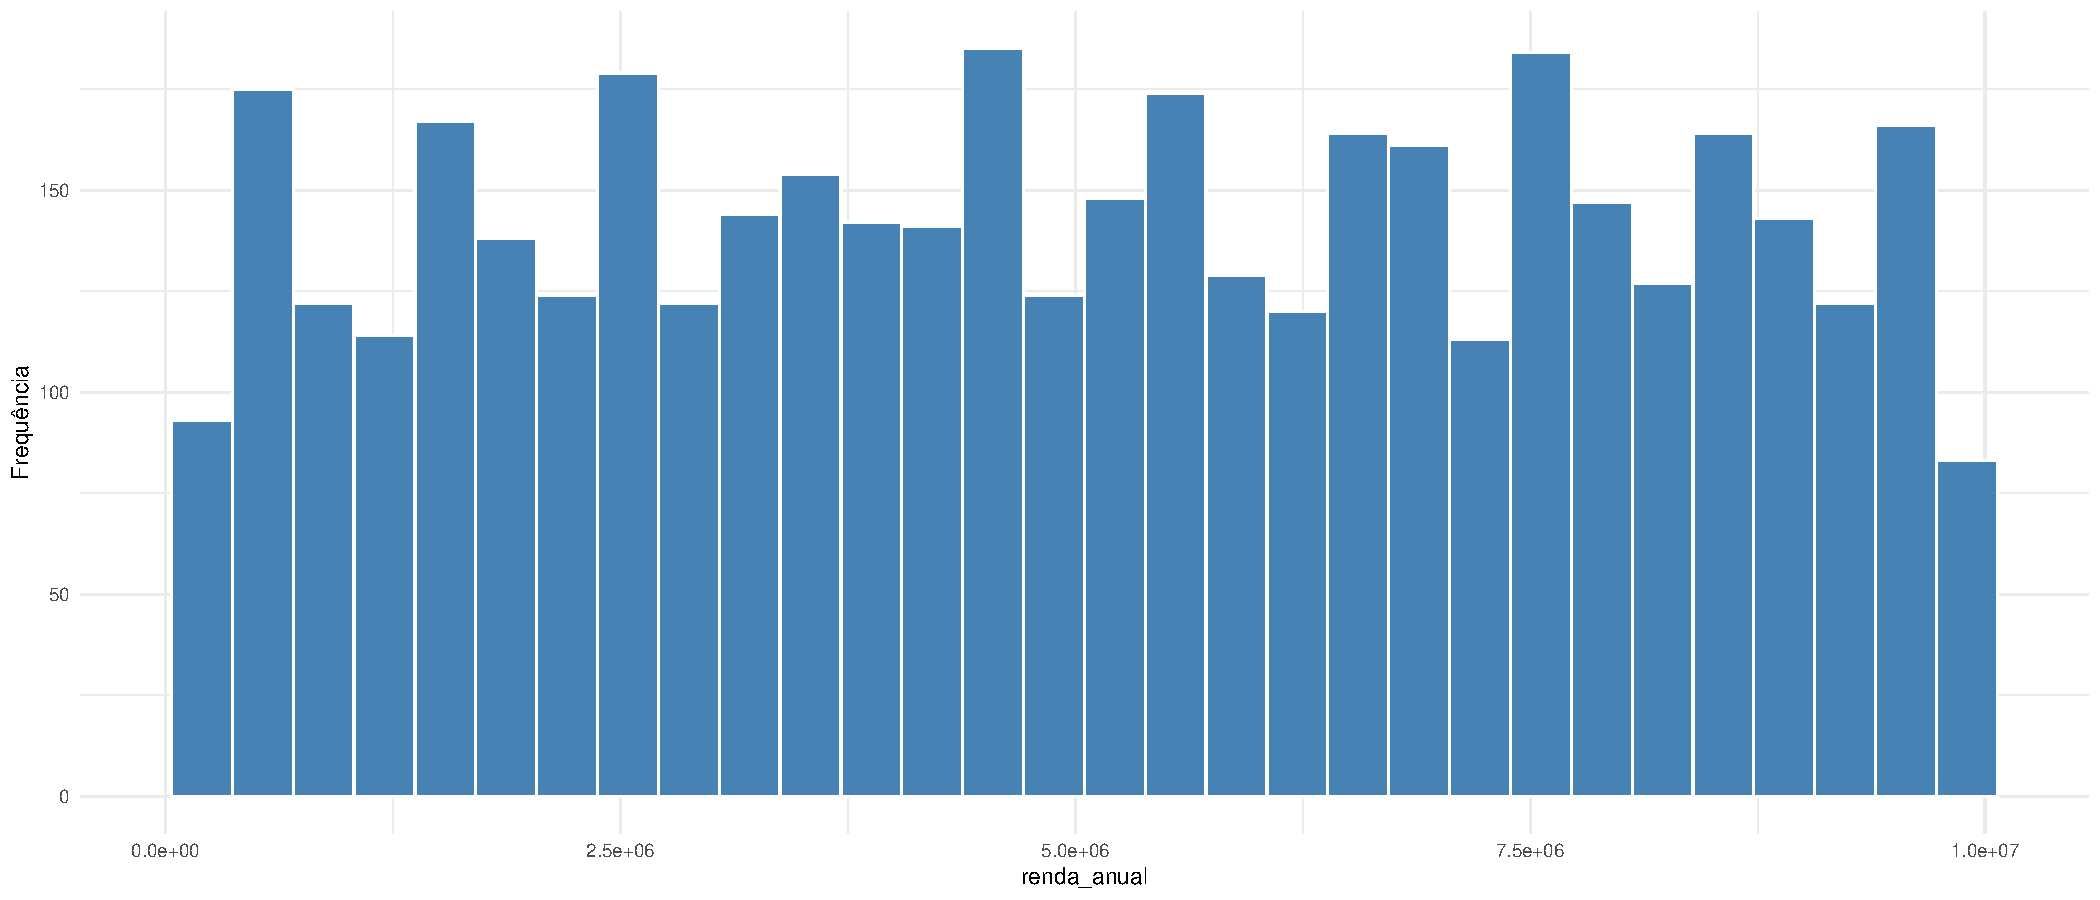
\includegraphics[width=1\linewidth,height=\textheight,keepaspectratio]{monografia_files/figure-pdf/fig-distribuicoes-1.pdf}

}

\subcaption{\label{fig-distribuicoes-1}Distribuição da renda anual}

\end{minipage}%
%
\begin{minipage}[t]{0.50\linewidth}

\centering{

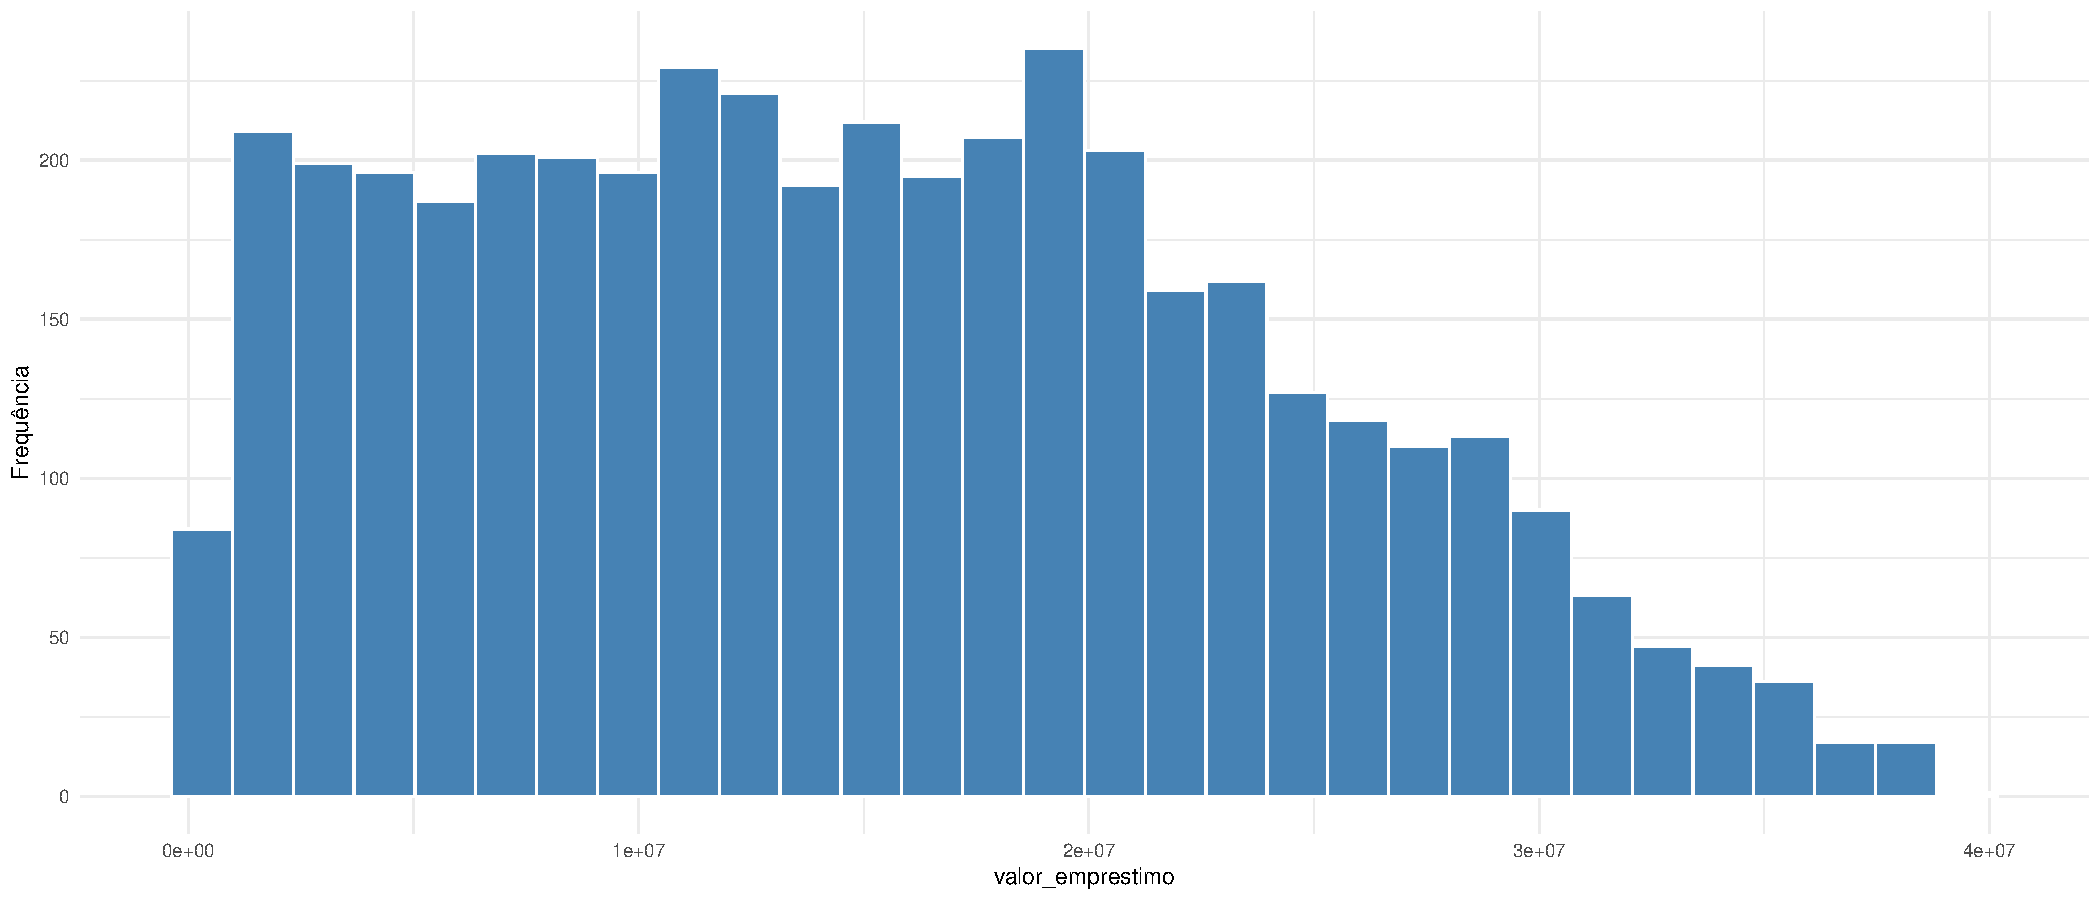
\includegraphics[width=1\linewidth,height=\textheight,keepaspectratio]{monografia_files/figure-pdf/fig-distribuicoes-2.pdf}

}

\subcaption{\label{fig-distribuicoes-2}Distribuição do valor do
empréstimo}

\end{minipage}%
\newline
\begin{minipage}[t]{0.50\linewidth}

\centering{

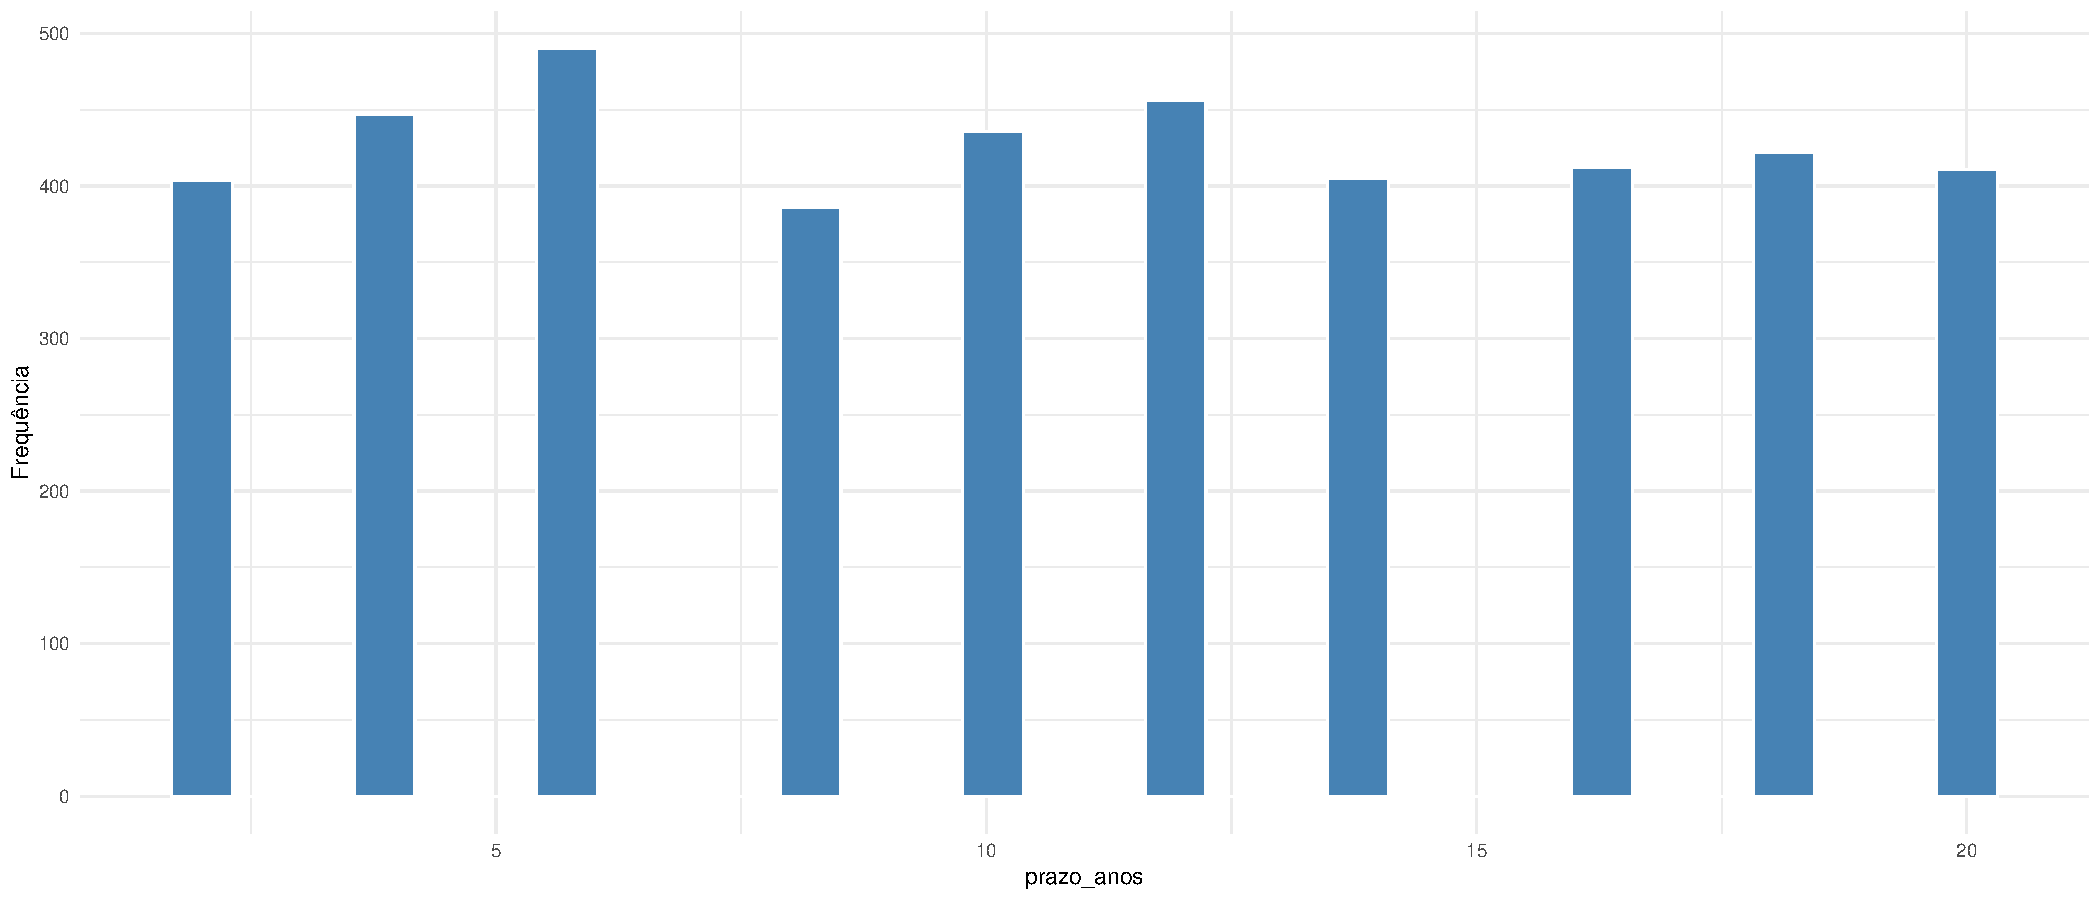
\includegraphics[width=1\linewidth,height=\textheight,keepaspectratio]{monografia_files/figure-pdf/fig-distribuicoes-3.pdf}

}

\subcaption{\label{fig-distribuicoes-3}Distribuição do prazo}

\end{minipage}%
%
\begin{minipage}[t]{0.50\linewidth}

\centering{

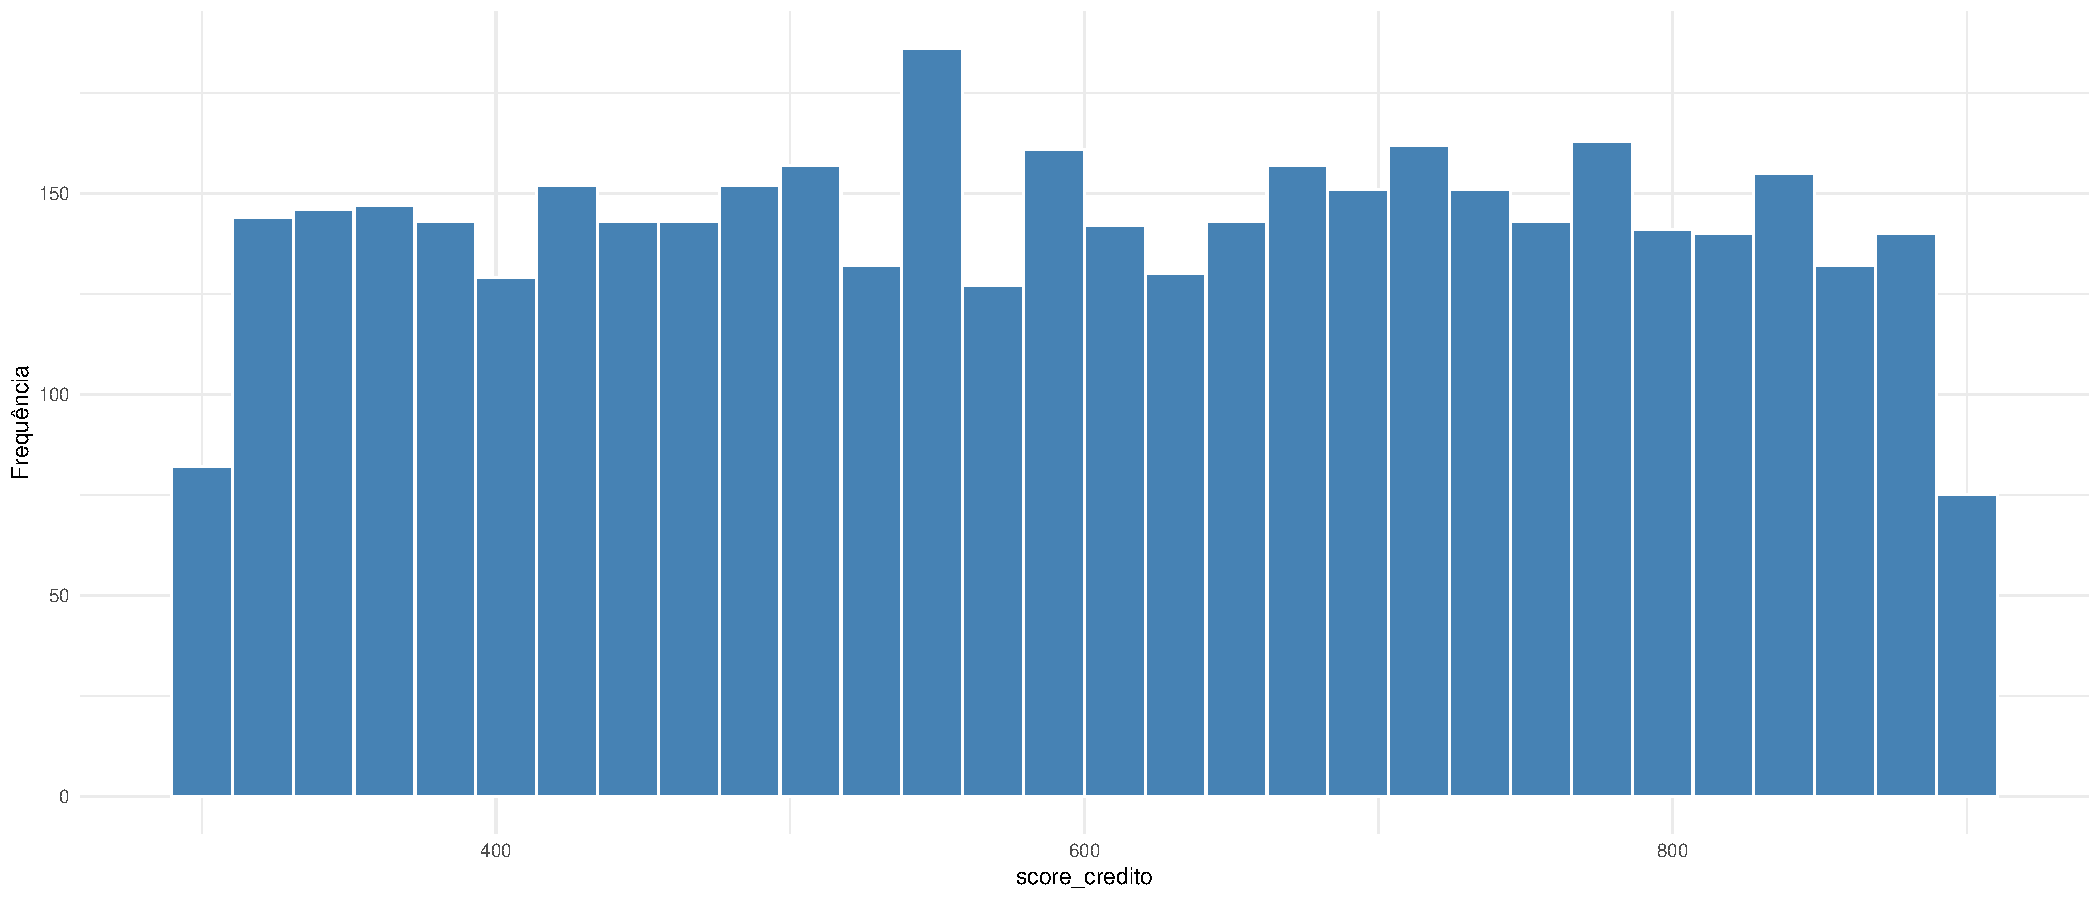
\includegraphics[width=1\linewidth,height=\textheight,keepaspectratio]{monografia_files/figure-pdf/fig-distribuicoes-4.pdf}

}

\subcaption{\label{fig-distribuicoes-4}Distribuição do CIBIL score}

\end{minipage}%
\newline
\begin{minipage}[t]{0.50\linewidth}

\centering{

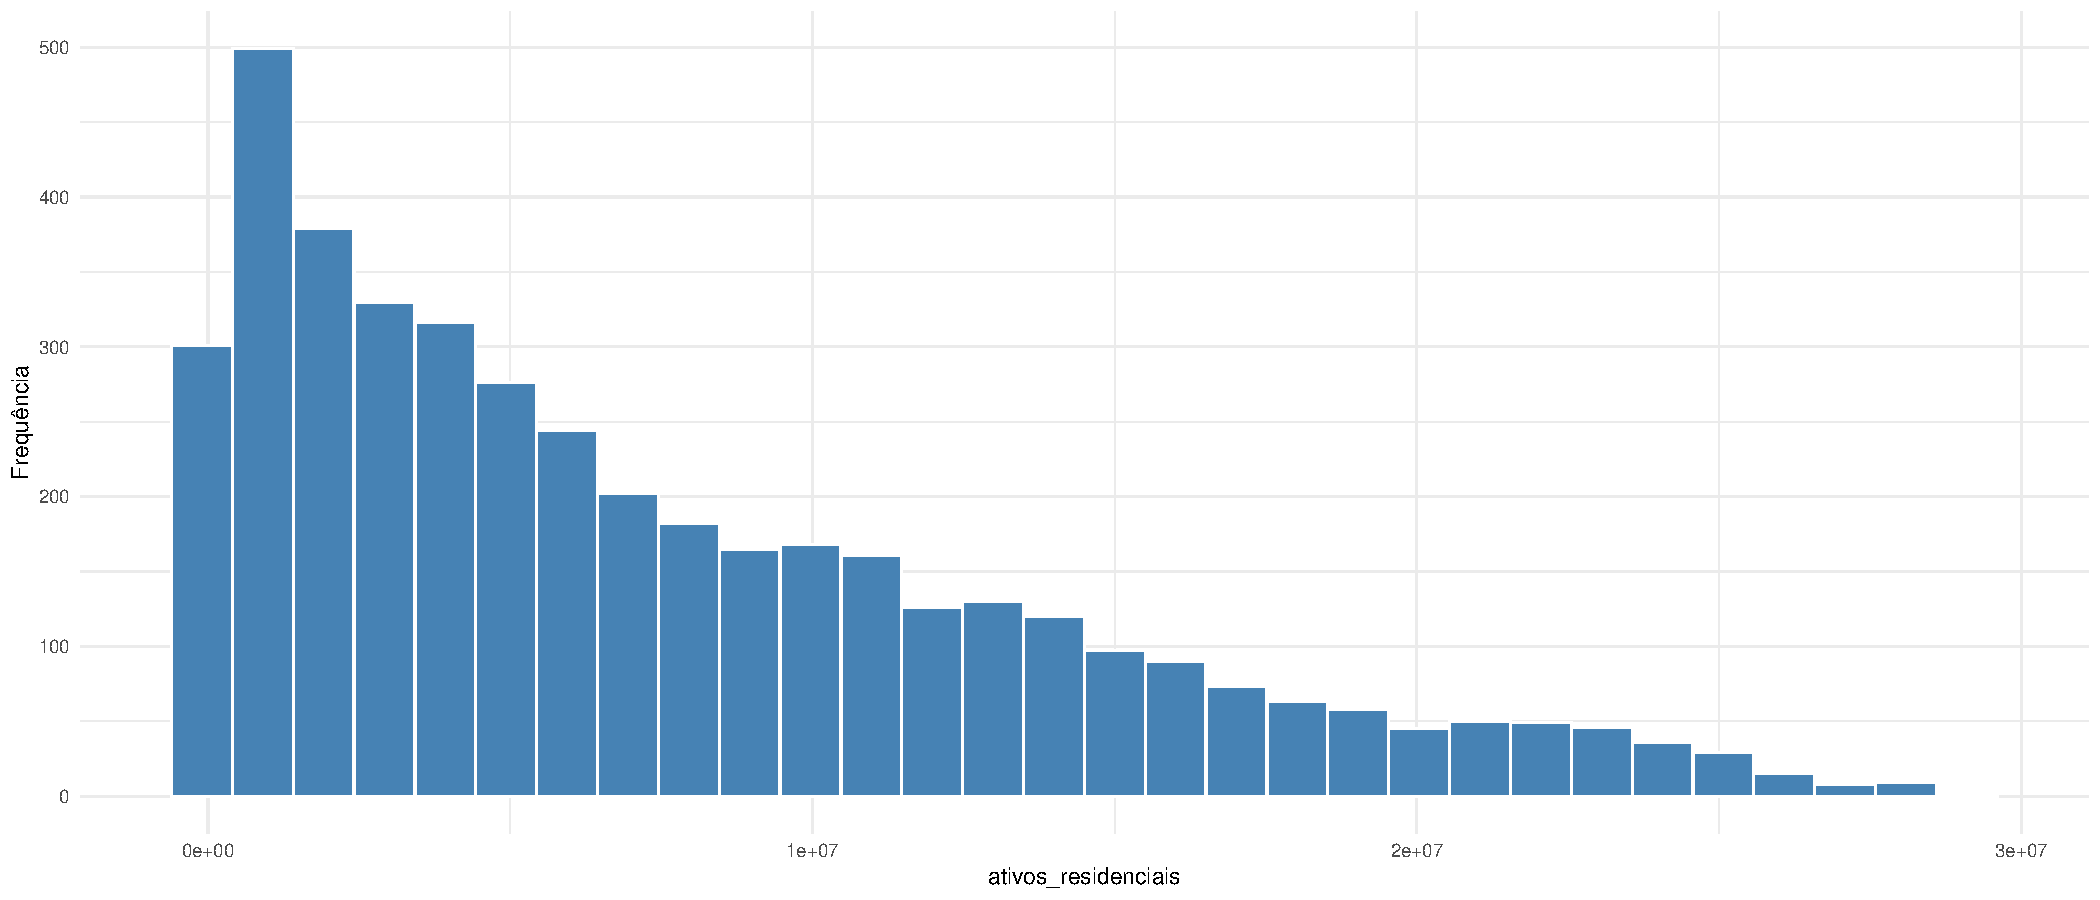
\includegraphics[width=1\linewidth,height=\textheight,keepaspectratio]{monografia_files/figure-pdf/fig-distribuicoes-5.pdf}

}

\subcaption{\label{fig-distribuicoes-5}Distribuição dos ativos
residenciais}

\end{minipage}%
%
\begin{minipage}[t]{0.50\linewidth}

\centering{

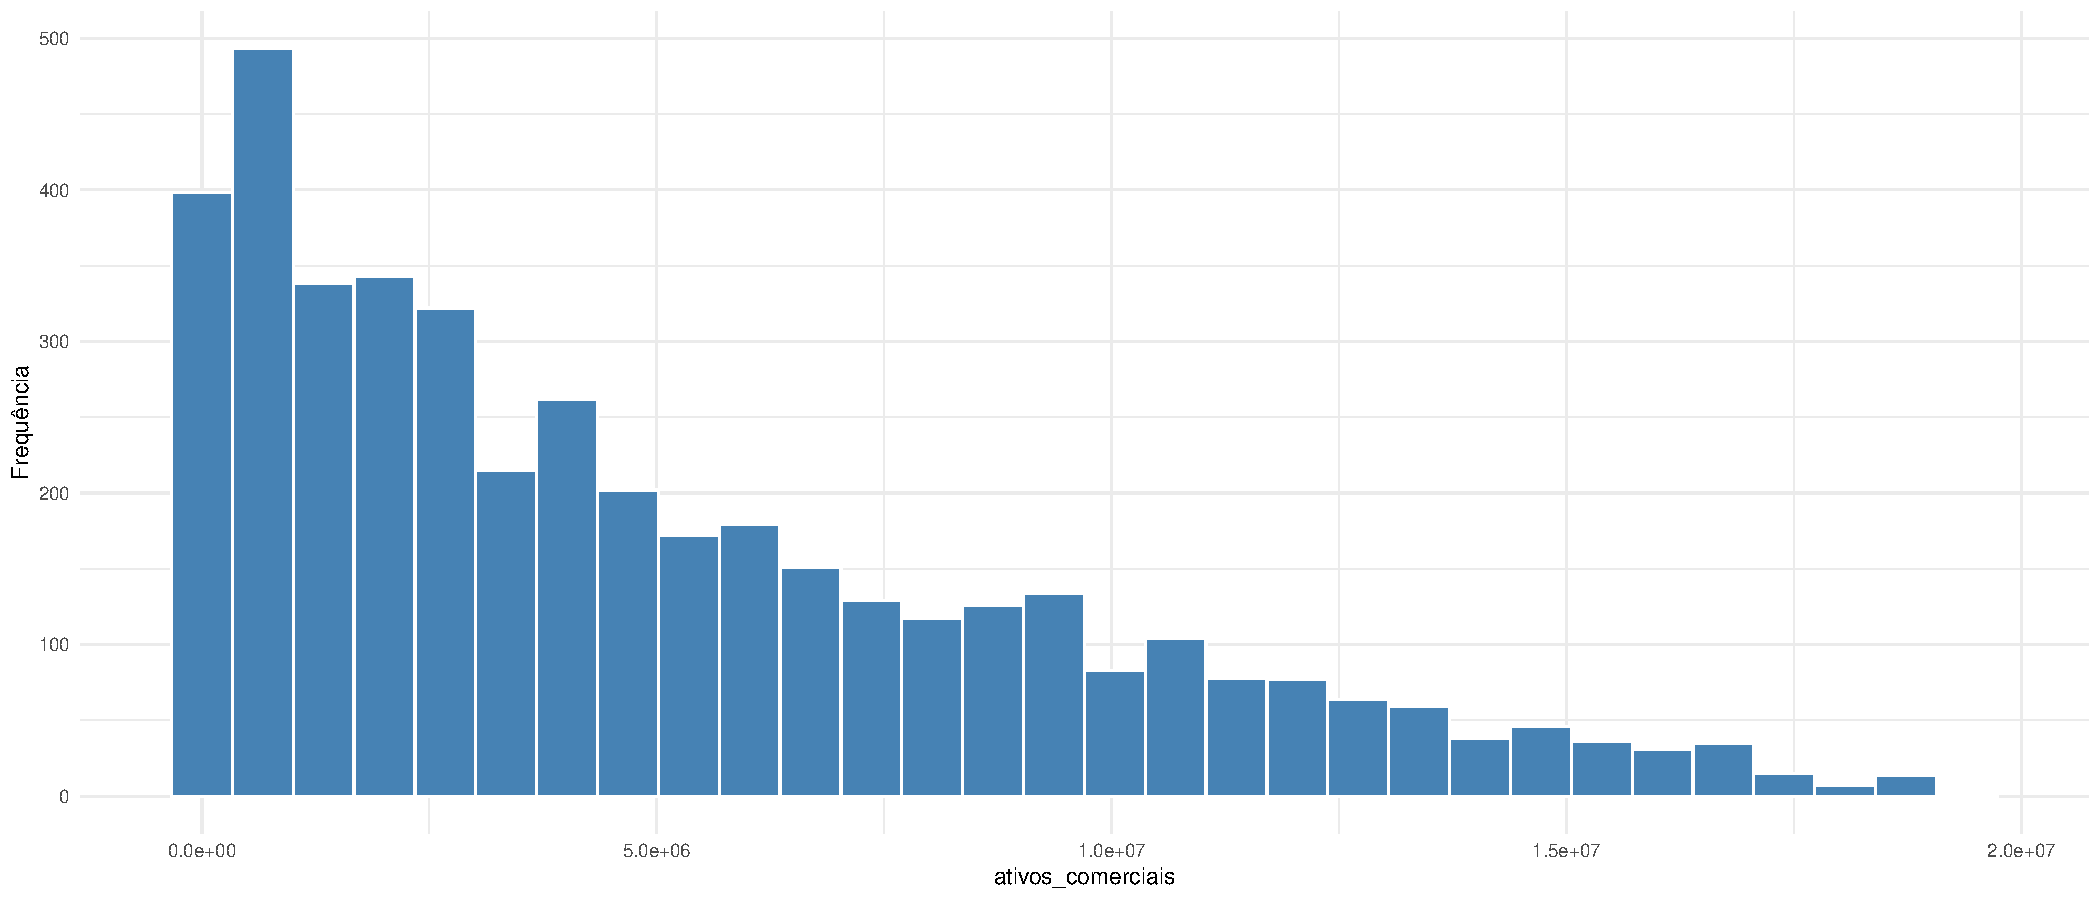
\includegraphics[width=1\linewidth,height=\textheight,keepaspectratio]{monografia_files/figure-pdf/fig-distribuicoes-6.pdf}

}

\subcaption{\label{fig-distribuicoes-6}Distribuição dos ativos
comerciais}

\end{minipage}%
\newline
\begin{minipage}[t]{0.50\linewidth}

\centering{

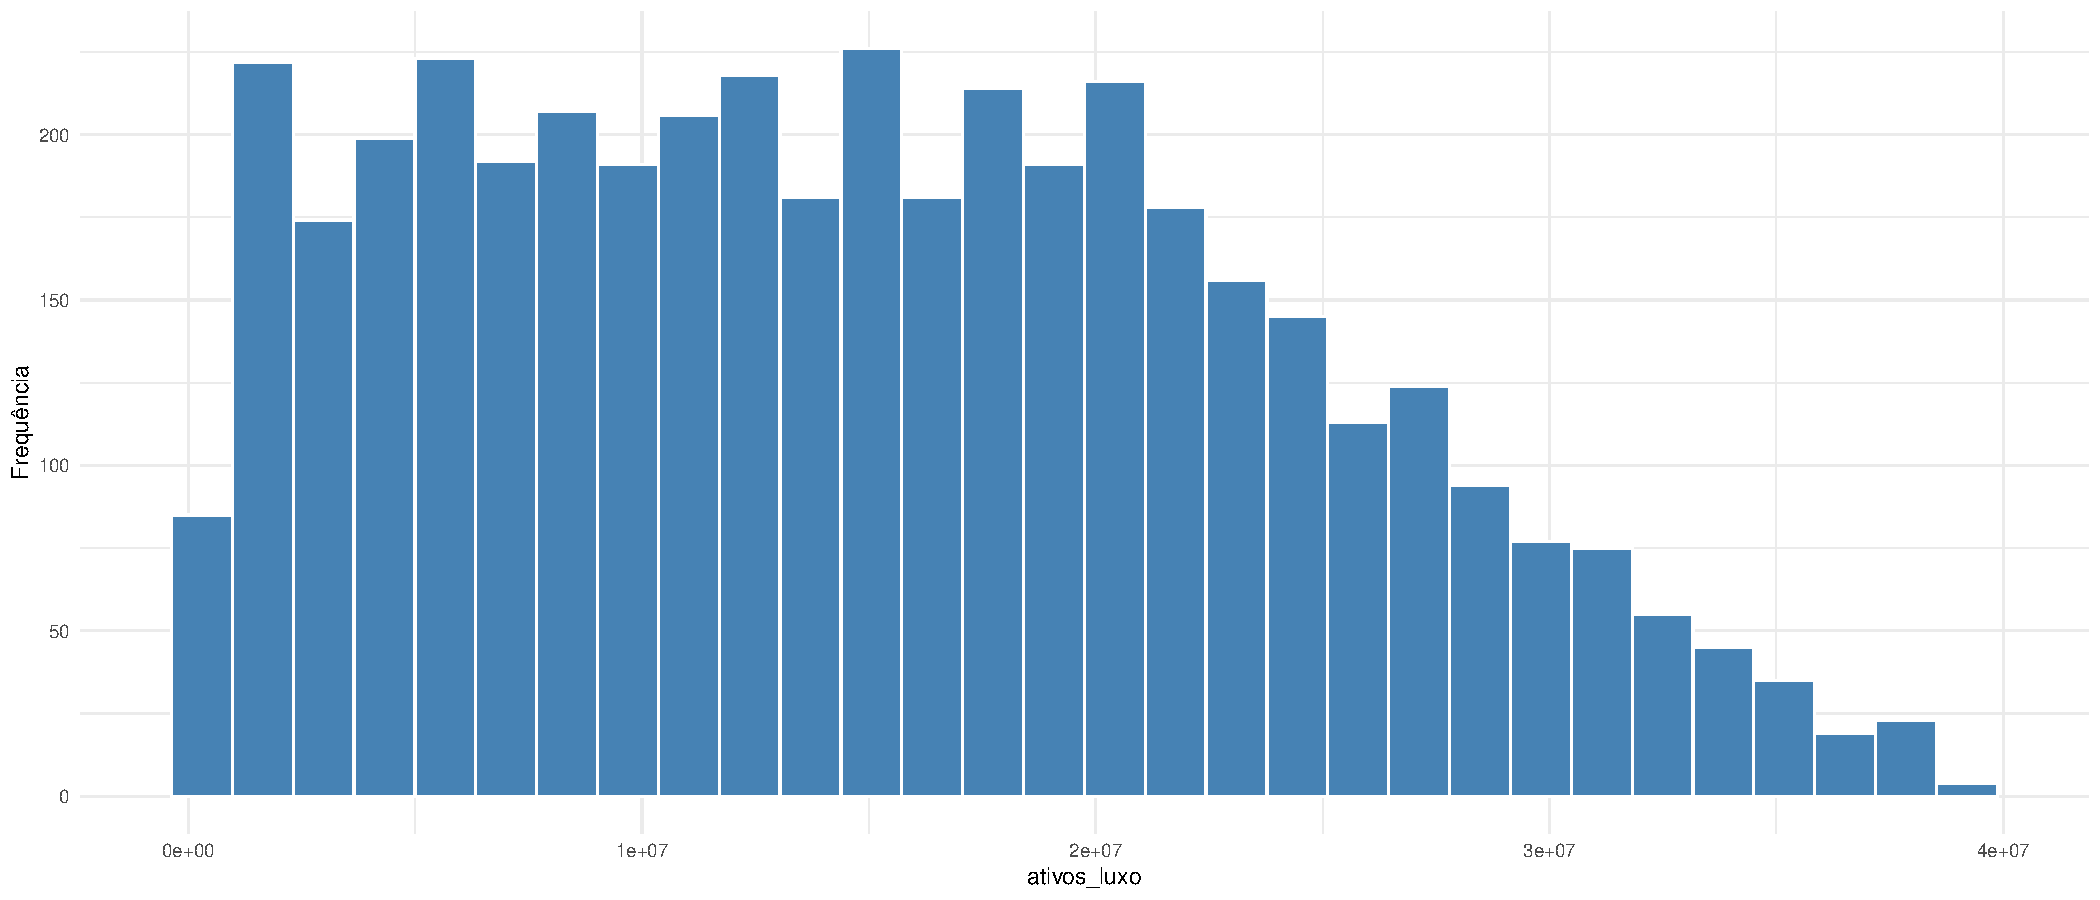
\includegraphics[width=1\linewidth,height=\textheight,keepaspectratio]{monografia_files/figure-pdf/fig-distribuicoes-7.pdf}

}

\subcaption{\label{fig-distribuicoes-7}Distribuição dos bens de luxo}

\end{minipage}%
%
\begin{minipage}[t]{0.50\linewidth}

\centering{

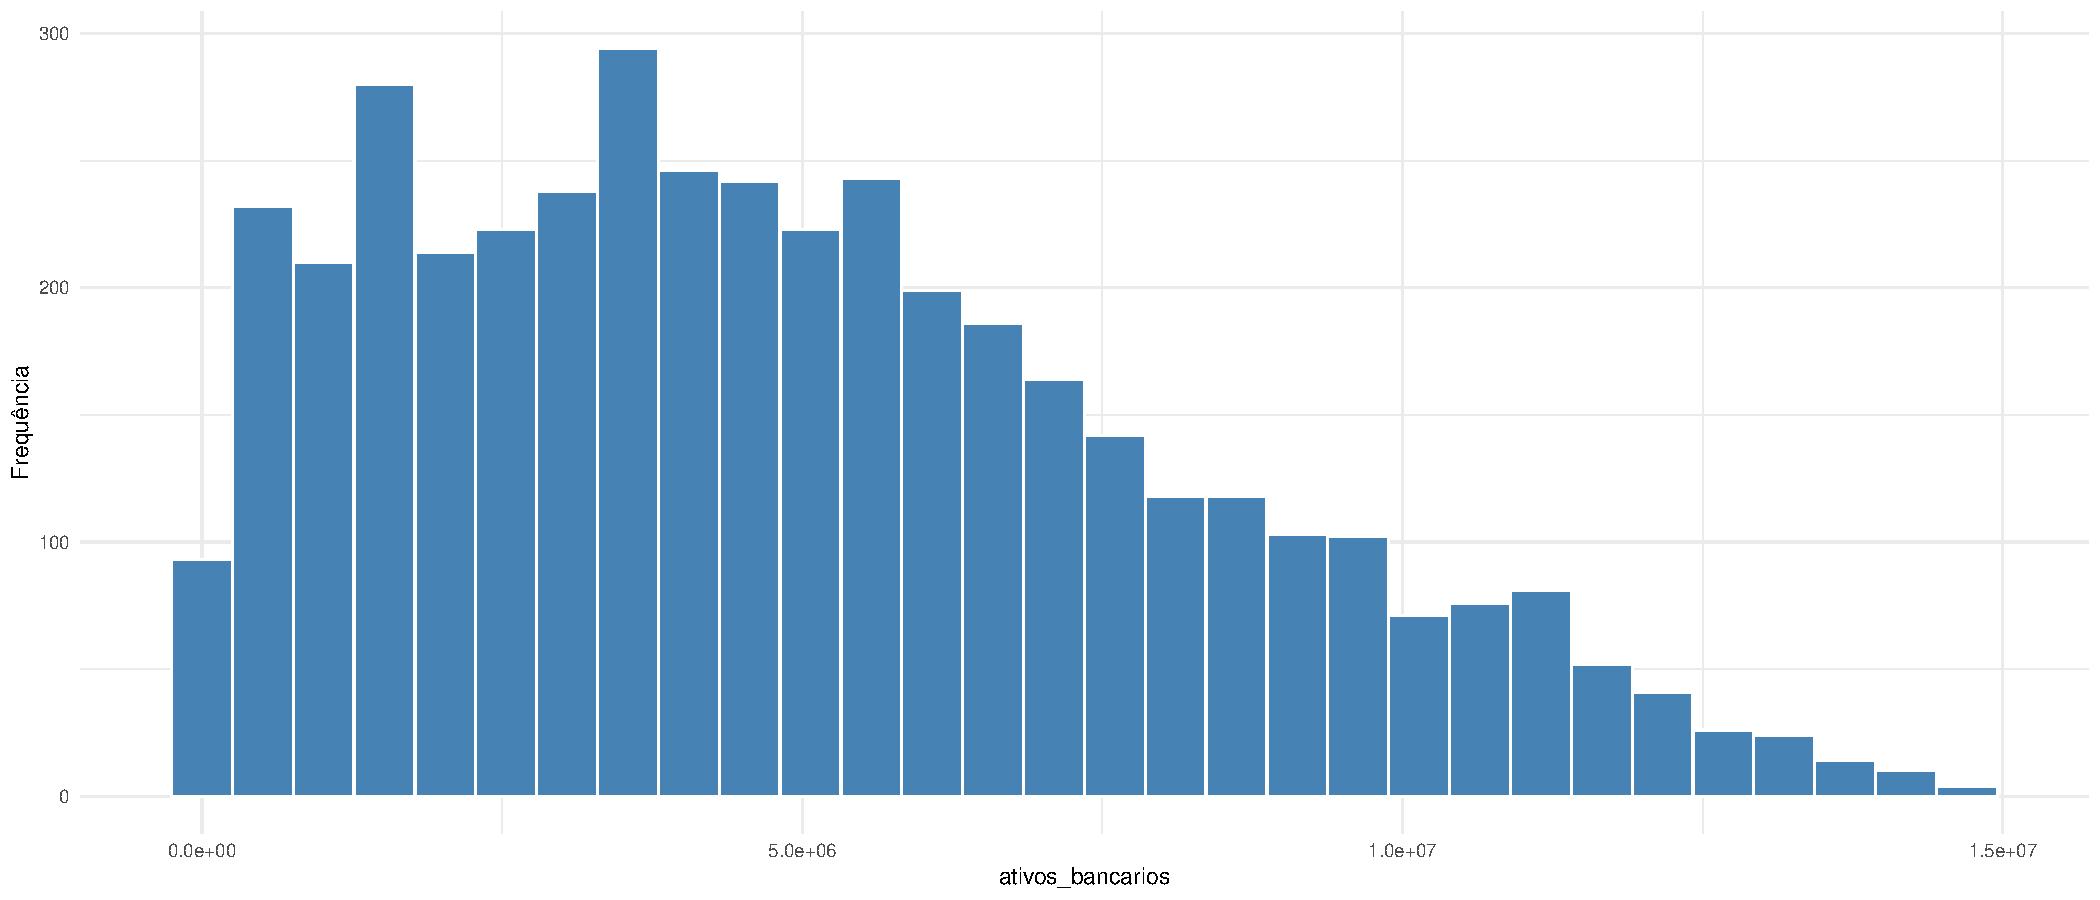
\includegraphics[width=1\linewidth,height=\textheight,keepaspectratio]{monografia_files/figure-pdf/fig-distribuicoes-8.pdf}

}

\subcaption{\label{fig-distribuicoes-8}Distribuição dos ativos
bancários}

\end{minipage}%

\caption{\label{fig-distribuicoes}Distribuição das principais variáveis
numéricas do conjunto de dados}

\end{figure}%

Na Figura~\ref{fig-distribuicoes} são apresentadas as distribuições das
variáveis numéricas analisadas. As variáveis (a) Renda Anual, (c) Prazo
do Empréstimo e (d) Score exibem distribuições relativamente homogêneas,
sem concentração acentuada em intervalos específicos. Esse padrão sugere
que o conjunto de dados contempla uma ampla variedade de perfis de
clientes, não havendo predominância excessiva de indivíduos com renda
muito elevada ou muito baixa, nem de faixas específicas de score de
crédito.

Para a variável Prazo do Empréstimo (c), observa-se a presença de picos
discretos ao longo da distribuição, o que é esperado, dado que prazos de
empréstimo são usualmente definidos em valores inteiros de anos.

Em contraste, as variáveis (e) Ativos Residenciais, (f) Ativos
Comerciais, (g) Bens de Luxo e (h) Ativos Bancários apresentam acentuada
assimetria à direita, indicando que a maioria dos indivíduos possui
ativos de menor valor, enquanto uma parcela reduzida concentra
patrimônios significativamente mais elevados.

\red{podemos tratar com transformações logarítmicas ou Box-Cox, mas deixei quieto por enquanto, usaria apenas na frequentista}

A (b) Distribuição do valor do empréstimo se mantém constante até um
certo patamar (em torno de 20 milhões) e depois sofre uma queda
acentuada. Indicando que o banco tem um limite de crédito comum para a
maioria dos clientes, e empréstimos acima desse valor são exceções ou
exigem critérios muito mais rígidos, tornando-os menos frequentes.

Outro ponto relevante é a presença de valores negativos em
\texttt{residential\_assets\_value}, como podemos ver em
Tabela~\ref{tbl-variaveis-num}, o que pode indicar inconsistências de
registro ou tratamentos contábeis específicos no conjunto de dados. Esse
tipo de característica pode afetar a modelagem, exigindo atenção em
etapas de pré-processamento.

A Tabela~\ref{tbl-categoricas} apresenta a distribuição das variáveis
categóricas do conjunto de dados. Observa-se que as categorias
analisadas exibem distribuições globalmente equilibradas, sem
predominância acentuada de um único grupo, o que contribui para a
estabilidade estatística e reduz potenciais vieses na etapa de
modelagem.

{

\begin{longtable}[]{@{}llrr@{}}

\caption{\label{tbl-categoricas}Distribuição das variáveis categóricas
do conjunto de dados.}

\tabularnewline

\toprule\noalign{}
variavel & categoria & n & percentual (\%) \\
\midrule\noalign{}
\endhead
\bottomrule\noalign{}
\endlastfoot
num\_dependentes & 0 & 712 & 16.68 \\
num\_dependentes & 1 & 697 & 16.33 \\
num\_dependentes & 2 & 708 & 16.58 \\
num\_dependentes & 3 & 727 & 17.03 \\
num\_dependentes & 4 & 752 & 17.62 \\
num\_dependentes & 5 & 673 & 15.76 \\
escolaridade & Graduate & 2144 & 50.22 \\
escolaridade & Not Graduate & 2125 & 49.78 \\
autonomo & No & 2119 & 49.64 \\
autonomo & Yes & 2150 & 50.36 \\

\end{longtable}

}

\paragraph{{[}REVISÃO-1{]} Análise da variável resposta e relações com
as variáveis
preditoras}\label{revisuxe3o-1-anuxe1lise-da-variuxe1vel-resposta-e-relauxe7uxf5es-com-as-variuxe1veis-preditoras}

Na Figura~\ref{fig-target-plot}, observa-se a distribuição da variável
resposta \texttt{status}, indicando que aproximadamente 62.22\% dos
empréstimos foram aprovados, enquanto 37.78\% foram rejeitados. Essa
proporção sugere um desequilíbrio leve na classe alvo.

\begin{figure}

\centering{

\pandocbounded{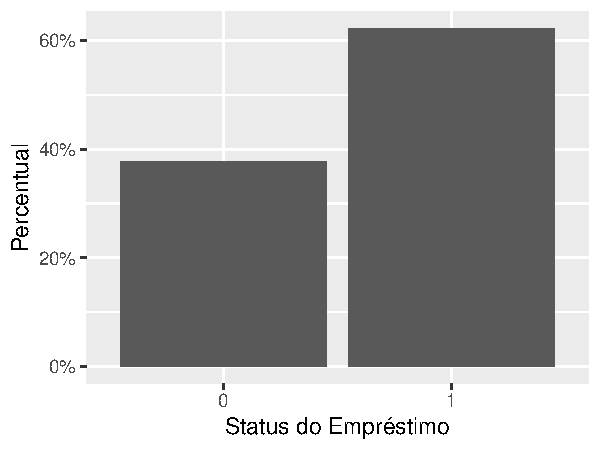
\includegraphics[keepaspectratio]{monografia_files/figure-pdf/fig-target-plot-1.pdf}}

}

\caption{\label{fig-target-plot}Distribuição da aprovação de
empréstimos}

\end{figure}%

A Figura~\ref{fig-distribuicoes-target} apresenta a estimativa de
densidade para as variáveis numéricas do conjunto de dados, segmentadas
pelo status de aprovação do empréstimo (Rejeitado ou Aprovado).
Observa-se que a variável \texttt{score\_credito} é a que apresenta a
separação mais nítida entre as classes: candidatos com scores mais
baixos (aproximadamente abaixo de 600) concentram-se majoritariamente no
grupo de rejeitados, enquanto scores elevados mostram uma densidade
quase exclusiva de aprovações.

No que tange ao prazo do empréstimo (\texttt{loan\_term}), nota-se uma
ligeira predominância de rejeições em prazos muito curtos, enquanto os
prazos mais longos apresentam uma distribuição mais equilibrada entre os
grupos. Em contraste, o restante das variáveis exibem distribuições
sobrepostas e visualmente semelhantes entre as duas classes. Tal
sobreposição indica que, isoladamente, essas variáveis possuem menor
poder discriminatório, o que exigirá dos modelos de regressão a
identificação de correlações mais complexas ou efeitos multivariados
para contribuir com a predição.

\begin{figure}

\centering{

\pandocbounded{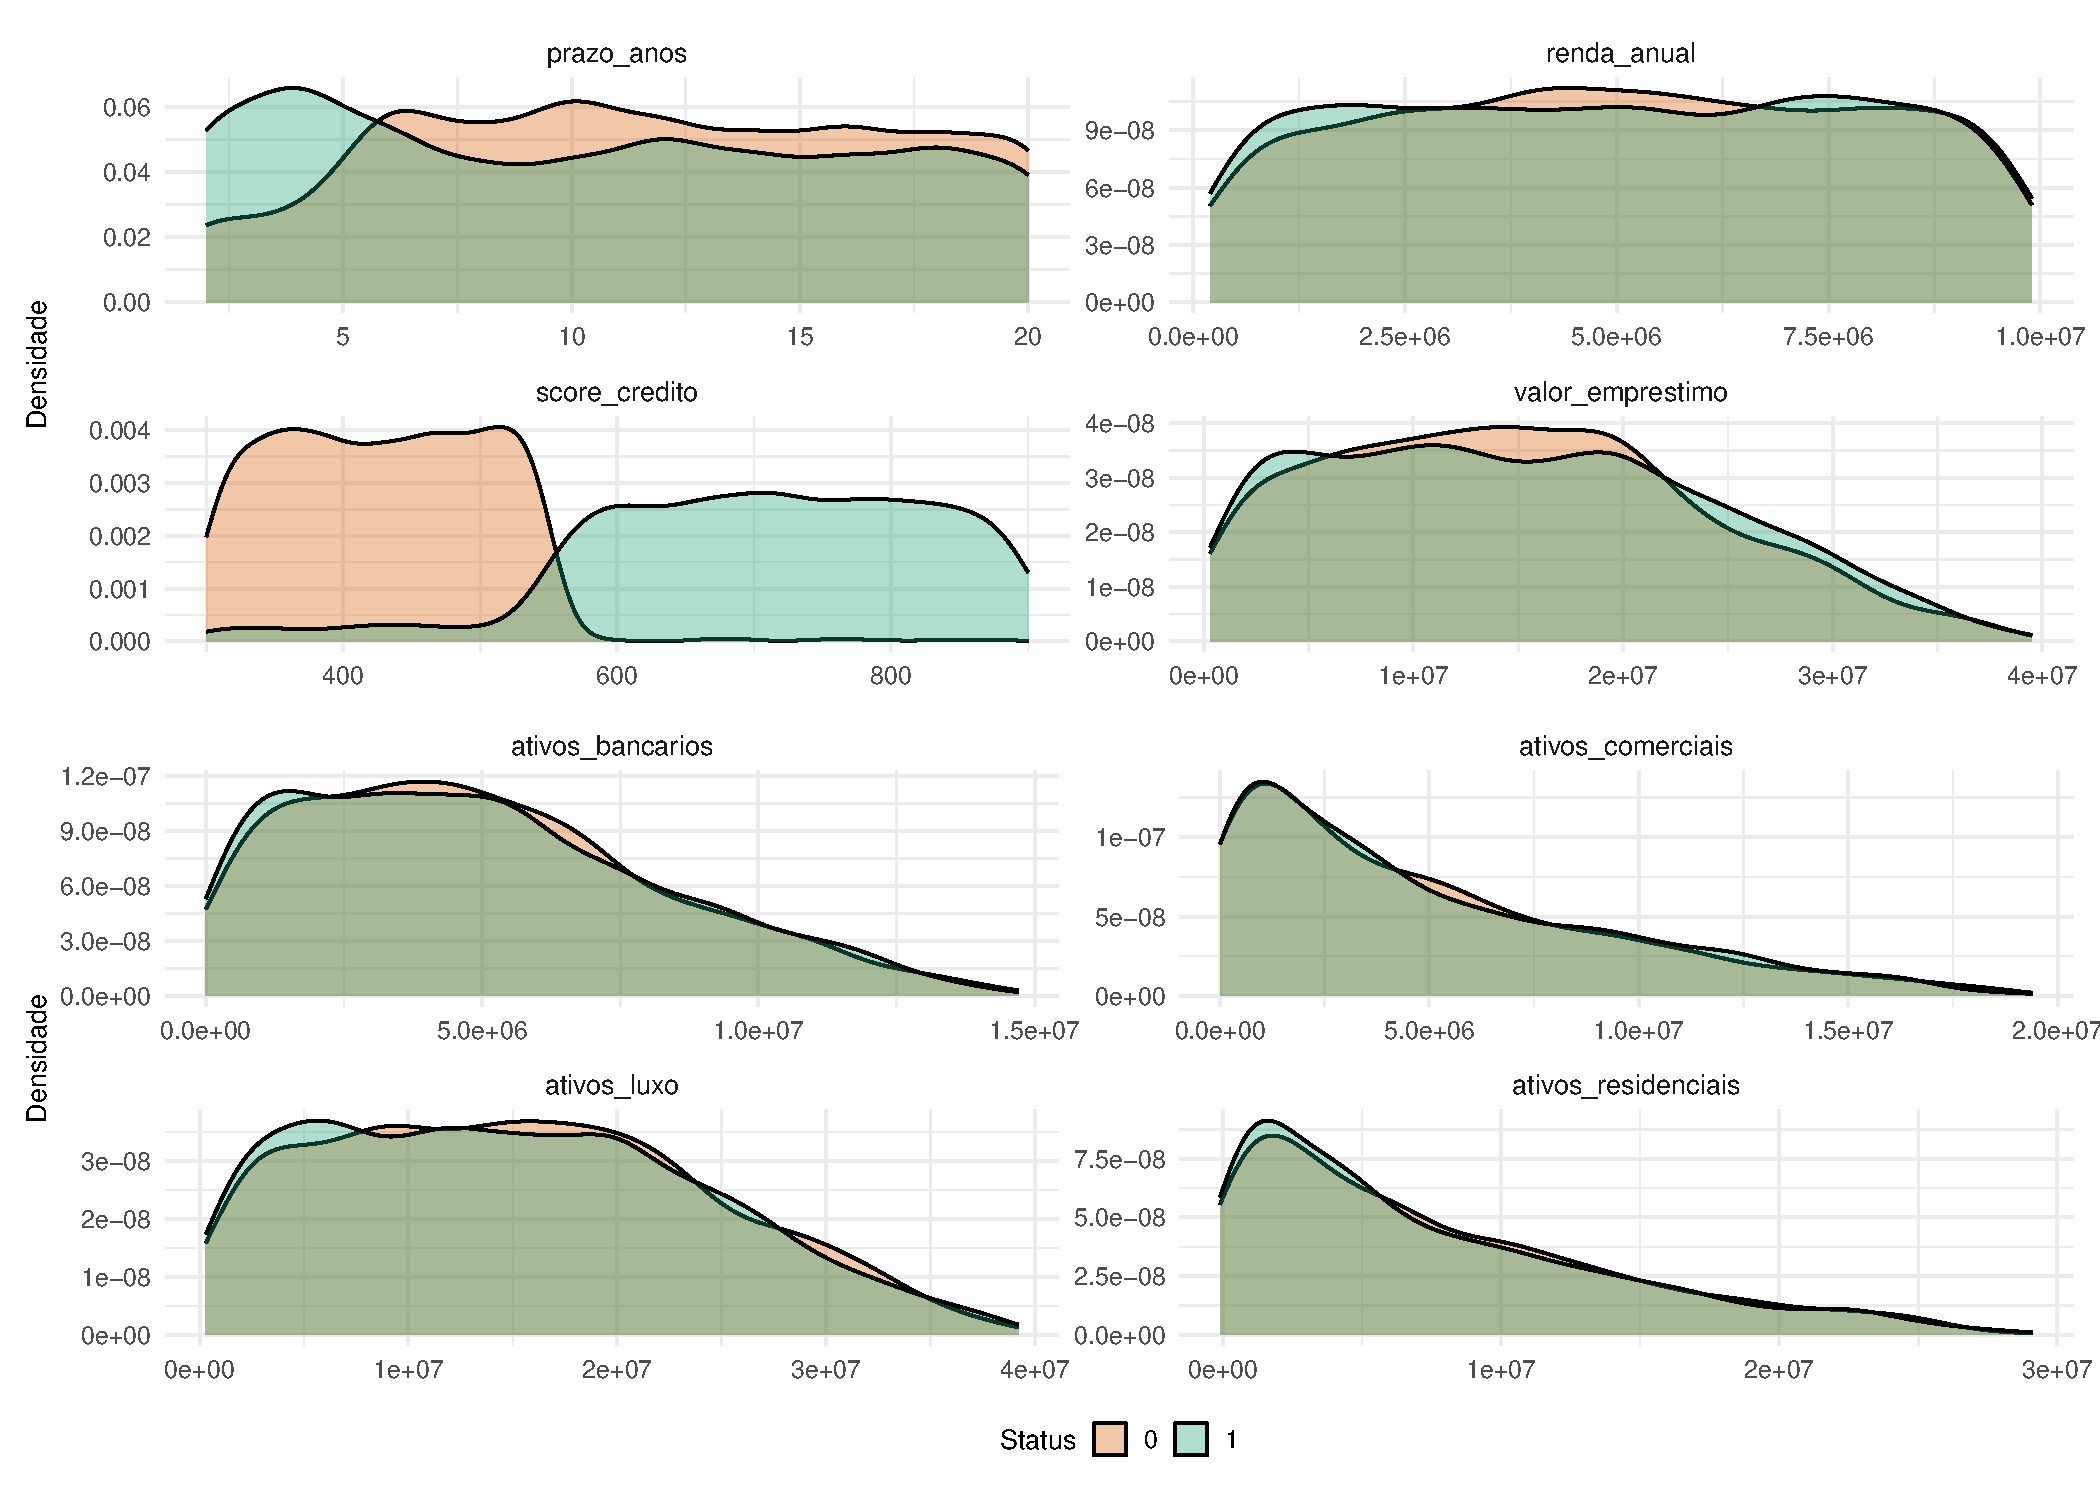
\includegraphics[keepaspectratio]{monografia_files/figure-pdf/fig-distribuicoes-target-1.pdf}}

}

\caption{\label{fig-distribuicoes-target}Distribuição das variáveis
numéricas por status de aprovação do empréstimo}

\end{figure}%

A Figura~\ref{fig-categoricas} apresenta a distribuição das frequências
absolutas para as variáveis categóricas Nível educacional, Trabalho
autônomo e Número de dependentes, segmentadas pelo status de aprovação.
Observa-se que a proporção entre empréstimos aprovados e rejeitados
mantém-se praticamente constante, independentemente de o candidato ser
graduado ou não, ou de possuir trabalho autônomo. No que tange ao número
de dependentes, o comportamento é análogo: não há uma categoria
específica (de 0 a 5 dependentes) que apresente uma vantagem ou
desvantagem desproporcional na aprovação do crédito. Sob a ótica da
modelagem estatística, essa independência aparente sugere que tais
variáveis podem apresentar coeficientes com menor magnitude ou maior
incerteza .

\begin{figure}

\centering{

\pandocbounded{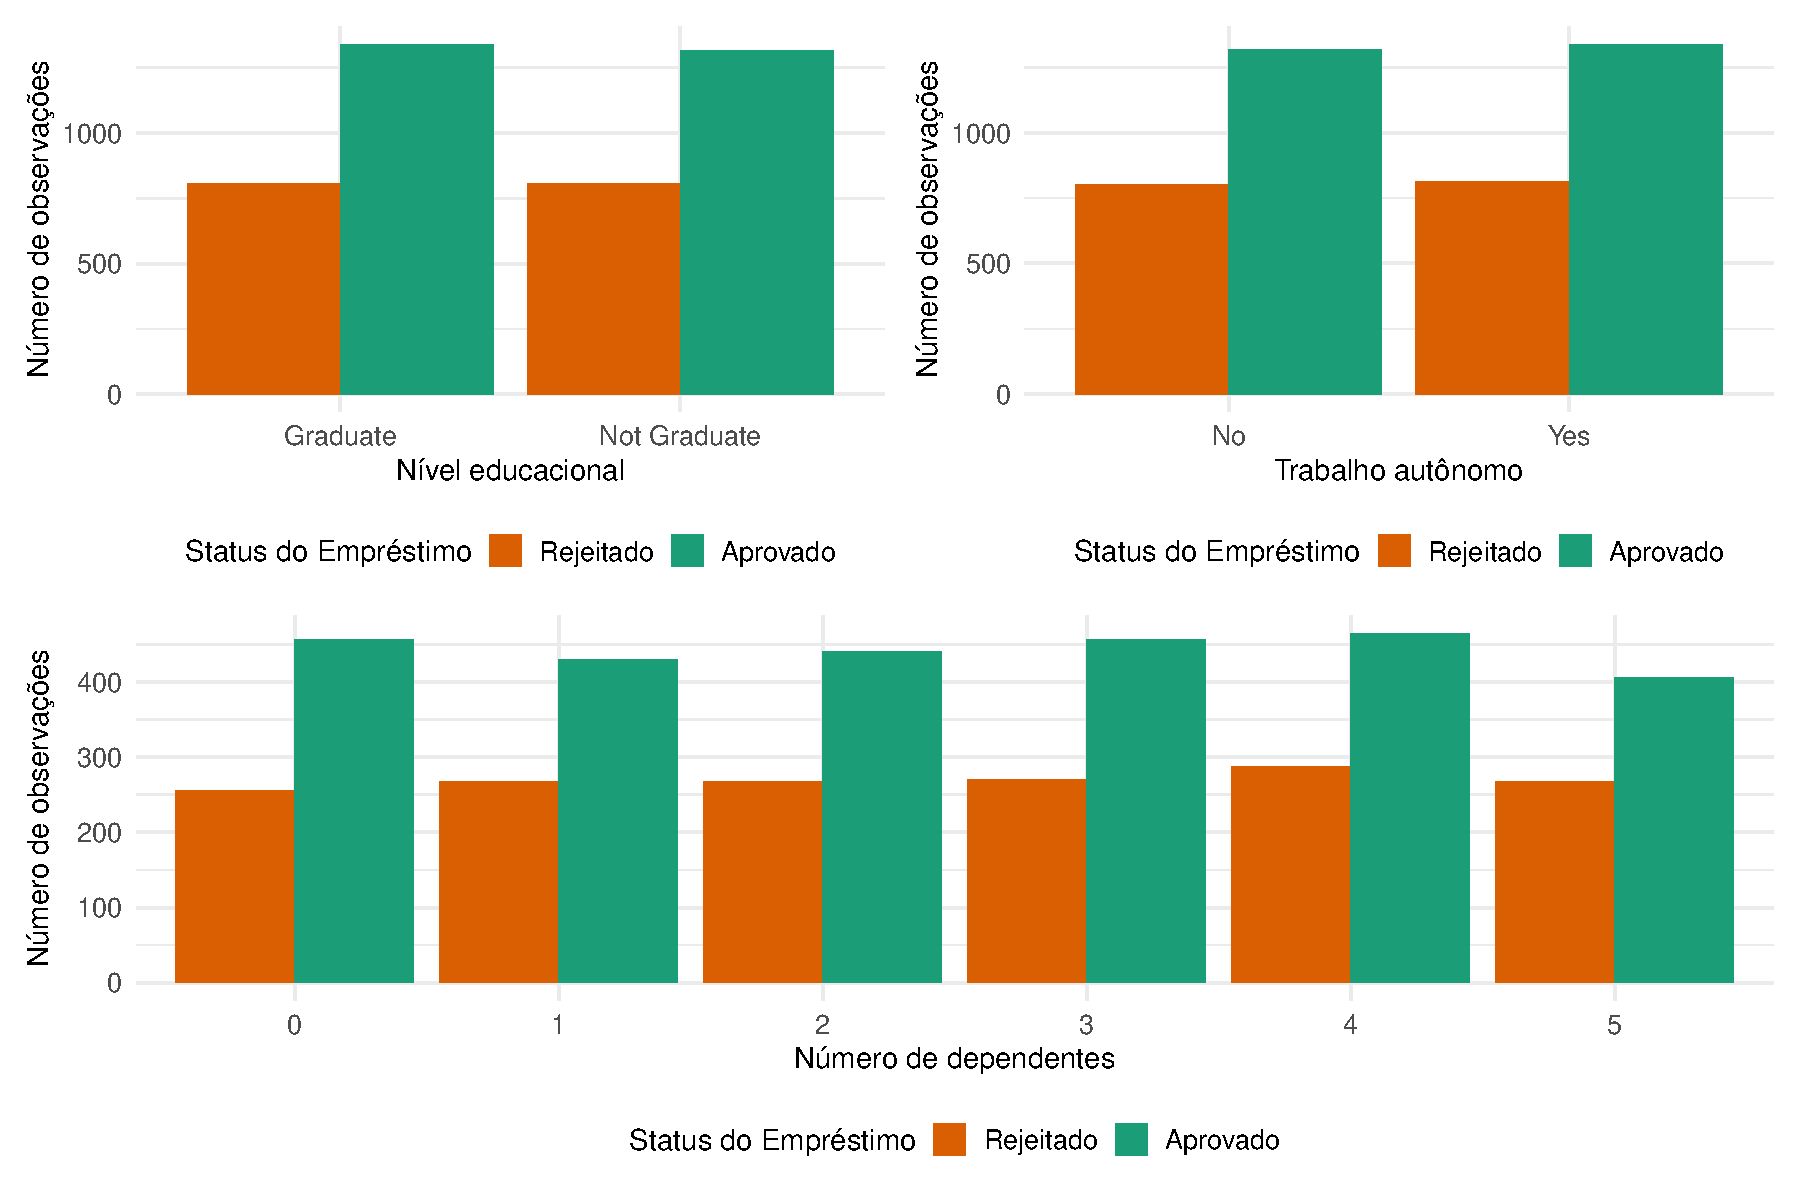
\includegraphics[keepaspectratio]{monografia_files/figure-pdf/fig-categoricas-1.pdf}}

}

\caption{\label{fig-categoricas}Distribuição das variáveis categóricas
segundo o status do empréstimo}

\end{figure}%

\paragraph{{[}REVISÃO-1{]} Análise de correlação entre variáveis
numéricas}\label{revisuxe3o-1-anuxe1lise-de-correlauxe7uxe3o-entre-variuxe1veis-numuxe9ricas}

A matriz de correlação (Figura~\ref{fig-correlacao}) revela associações
relevantes entre as variáveis numéricas do conjunto de dados. Observa-se
forte correlação entre renda anual e valor do empréstimo, bem como entre
essas variáveis e os ativos patrimoniais, especialmente ativos de luxo e
ativos bancários, indicando que essas medidas capturam aspectos
relacionados da condição financeira dos solicitantes. As correlações
entre os diferentes tipos de ativos são positivas e moderadas, sugerindo
coerência interna do perfil patrimonial, sem redundância perfeita entre
as variáveis.

Por outro lado, o prazo do empréstimo apresenta correlação praticamente
nula com as demais variáveis, indicando independência em relação ao
perfil financeiro. De forma semelhante, o score\_credito exibe
correlações muito fracas com renda, ativos e valor do empréstimo,
sugerindo que essa variável representa uma dimensão distinta de risco de
crédito, relevante para a classificação, mas não diretamente associada
ao nível de riqueza.

A presença de correlações elevadas entre algumas variáveis explicativas
indica potencial multicolinearidade, aspecto que deve ser considerado na
etapa de modelagem, especialmente na interpretação dos coeficientes da
regressão logística.

\begin{figure}[htbp]

\centering{

\pandocbounded{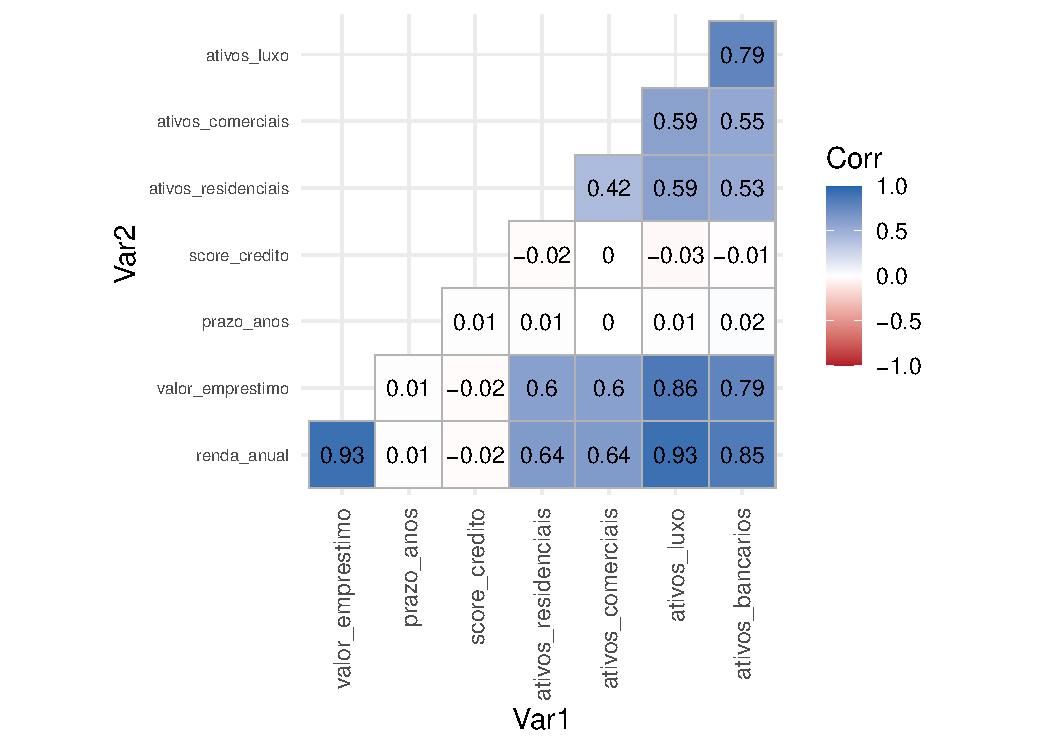
\includegraphics[keepaspectratio]{monografia_files/figure-pdf/fig-correlacao-1.pdf}}

}

\caption{\label{fig-correlacao}Mapa de calor da correlação entre
variáveis numéricas}

\end{figure}%

\paragraph{{[}REVISÃO-1{]} Análise de
outliers}\label{revisuxe3o-1-anuxe1lise-de-outliers}

A presença de valores atípicos, particularmente em variáveis
relacionadas a ativos patrimoniais, é corroborada quantitativamente pela
Tabela~\ref{tbl-outliers}, que apresenta o número e o percentual de
observações classificadas como outliers segundo o critério do intervalo
interquartil. Esses valores extremos refletem a heterogeneidade típica
de dados financeiros e possuem implicações diretas para a modelagem
estatística. Enquanto abordagens frequentistas podem demandar
procedimentos de tratamento ou estimadores robustos para mitigar a
influência desses pontos, modelos bayesianos permitem incorporar
explicitamente essa incerteza por meio de distribuições com caudas mais
pesadas, oferecendo maior flexibilidade na avaliação do impacto dos
outliers sobre os parâmetros estimados.

{

\begin{longtable}[]{@{}lrr@{}}

\caption{\label{tbl-outliers}Número e percentual de outliers
identificados pelo critério do IQR}

\tabularnewline

\toprule\noalign{}
Feature & Outliers & Percentual \\
\midrule\noalign{}
\endhead
\bottomrule\noalign{}
\endlastfoot
ativos\_bancarios & 5 & 0.0011712 \\
ativos\_comerciais & 37 & 0.0086671 \\
ativos\_luxo & 0 & 0.0000000 \\
ativos\_residenciais & 52 & 0.0121808 \\
prazo\_anos & 0 & 0.0000000 \\
renda\_anual & 0 & 0.0000000 \\
score\_credito & 0 & 0.0000000 \\
valor\_emprestimo & 0 & 0.0000000 \\

\end{longtable}

}

\paragraph{{[}REVISÃO-1{]} Pré
processamento}\label{revisuxe3o-1-pruxe9-processamento-1}

\subparagraph{{[}REVISÃO-1{]} Verificação de valores ausentes e
observações
duplicadas}\label{revisuxe3o-1-verificauxe7uxe3o-de-valores-ausentes-e-observauxe7uxf5es-duplicadas}

Inicialmente, foi realizada a verificação da presença de valores
ausentes e observações duplicadas no conjunto de dados. Não foram
identificados valores faltantes em nenhuma das variáveis, o que
dispensou a aplicação de técnicas de imputação e evitou a introdução de
incerteza adicional ou viés sistemático no processo de modelagem.
Adicionalmente, não foram detectadas observações duplicadas, assegurando
que cada registro corresponda a uma unidade amostral distinta e
contribuindo para a validade das estimativas inferenciais.

\paragraph{{[}REVISÃO-1{]} Tratamento de inconsistências e
outliers}\label{revisuxe3o-1-tratamento-de-inconsistuxeancias-e-outliers}

Observa-se que aproximadamente 0.01\% dos solicitantes apresentam
valores negativos para ativos residenciais, correspondendo a um
contingente residual de observações atípicas. Esses valores não possuem
interpretação econômica direta no contexto da variável analisada e podem
estar associados a inconsistências de registro ou a particularidades não
representativas do perfil financeiro da amostra. Considerando o caráter
marginal dessas observações e seu potencial de introduzir ruído na
estimação dos parâmetros, optou-se por removê-las do conjunto de dados,
sem prejuízo à representatividade da amostra ou à validade inferencial
dos modelos ajustados. A exclusão resultou na remoção de 28 observações.

Não foi aplicado tratamento automático de outliers, uma vez que valores
extremos são esperados em dados financeiros e podem conter informação
relevante para a classificação do risco de crédito.

\paragraph{{[}REVISÃO-1{]} Seleção de variáveis e análise de
correlação}\label{revisuxe3o-1-seleuxe7uxe3o-de-variuxe1veis-e-anuxe1lise-de-correlauxe7uxe3o}

A Figura~\ref{fig-correlacao} foi utilizada para investigar possíveis
relações de dependência linear entre as variáveis numéricas. Observou-se
a presença de correlações elevadas entre variáveis associadas à escala
de renda e patrimônio, como renda anual, valor do empréstimo e ativos
financeiros, comportamento esperado em bases de dados financeiras.

Apesar dessas correlações, optou-se por não remover variáveis nesta
etapa, mantendo todas as variáveis numéricas disponíveis para a
modelagem. Essa decisão foi motivada pelo interesse em avaliar o impacto
de cada variável no modelo de regressão logística.

\subsubsection{Dataset de
Inadimplência}\label{dataset-de-inadimpluxeancia}

O conjunto de dados de inadimplência é composto por 30000 observações e
25 variáveis, incluindo a variável resposta \texttt{PD30}, que indica se
As variáveis preditoras incluem informações como renda anual, pontuação
de crédito, nível educacional, entre outras características dos
solicitantes.

\paragraph{{[}WIP{]} Estatísticas
univariadas}\label{wip-estatuxedsticas-univariadas}

A Tabela~\ref{tbl-variaveis-num-default} evidencia uma população
heterogênea de clientes de cartão de crédito, com ampla variabilidade
tanto nas características demográficas quanto nas variáveis financeiras,
o que também pode ser visto no dataset de empretimos. O limite médio de
crédito é de aproximadamente NT\$ 167 mil, com mediana inferior (NT\$
140 mil), indicando assimetria à direita e a presença de clientes com
limites substancialmente mais elevados, o que é reforçado pelo alto
desvio padrão. A idade média dos clientes é de cerca de 35 anos, com
concentração em adultos jovens e de meia-idade. As variáveis categóricas
codificadas numericamente, como sexo, escolaridade e estado civil,
apresentam baixa variabilidade relativa, refletindo uma distribuição
razoavelmente equilibrada entre suas categorias principais.

No que diz respeito ao comportamento de pagamento, as variáveis de
atraso (\texttt{atraso\_pagto\_0} a \texttt{atraso\_pagto\_6})
apresentam médias próximas de zero e medianas iguais a zero, sugerindo
que a maioria dos clientes não apresenta atraso significativo nos
pagamentos, embora existam casos extremos de inadimplência prolongada
(até oito meses). Os valores de fatura e de pagamento exibem grande
dispersão (que pode ser vista na
Figura~\ref{fig-distribuicoes-default}), com médias substancialmente
superiores às medianas, o que indica distribuições fortemente
assimétricas e a presença de outliers. Ademais, a ocorrência de valores
negativos nas faturas é consistente com ajustes, estornos ou créditos no
sistema de faturamento. Em conjunto, esses resultados reforçam a
complexidade do perfil financeiro dos clientes e justificam o uso de
técnicas de modelagem robustas à assimetria, à presença de valores
extremos e à heterogeneidade dos dados monetários expressos em dólares
taiwaneses (NT\$).

{

\begin{longtable}[]{@{}
  >{\raggedright\arraybackslash}p{(\linewidth - 10\tabcolsep) * \real{0.2133}}
  >{\raggedleft\arraybackslash}p{(\linewidth - 10\tabcolsep) * \real{0.1467}}
  >{\raggedleft\arraybackslash}p{(\linewidth - 10\tabcolsep) * \real{0.1333}}
  >{\raggedleft\arraybackslash}p{(\linewidth - 10\tabcolsep) * \real{0.1200}}
  >{\raggedleft\arraybackslash}p{(\linewidth - 10\tabcolsep) * \real{0.2400}}
  >{\raggedleft\arraybackslash}p{(\linewidth - 10\tabcolsep) * \real{0.1467}}@{}}

\caption{\label{tbl-variaveis-num-default}Estatísticas descritivas das
variáveis numéricas do conjunto de dados.}

\tabularnewline

\toprule\noalign{}
\begin{minipage}[b]{\linewidth}\raggedright
\end{minipage} & \begin{minipage}[b]{\linewidth}\raggedleft
mean
\end{minipage} & \begin{minipage}[b]{\linewidth}\raggedleft
median
\end{minipage} & \begin{minipage}[b]{\linewidth}\raggedleft
min
\end{minipage} & \begin{minipage}[b]{\linewidth}\raggedleft
max
\end{minipage} & \begin{minipage}[b]{\linewidth}\raggedleft
std
\end{minipage} \\
\midrule\noalign{}
\endhead
\bottomrule\noalign{}
\endlastfoot
limite\_credito & 167484 & 140000 & 10000 & 1e+06 & 129748 \\
sexo & 1.6 & 2 & 1 & 2 & 0.49 \\
escolaridade & 1.85 & 2 & 0 & 6 & 0.79 \\
estado\_civil & 1.55 & 2 & 0 & 3 & 0.52 \\
idade & 35.49 & 34 & 21 & 79 & 9.22 \\
atraso\_pagto\_0 & -0.02 & 0 & -2 & 8 & 1.12 \\
atraso\_pagto\_2 & -0.13 & 0 & -2 & 8 & 1.2 \\
atraso\_pagto\_3 & -0.17 & 0 & -2 & 8 & 1.2 \\
atraso\_pagto\_4 & -0.22 & 0 & -2 & 8 & 1.17 \\
atraso\_pagto\_5 & -0.27 & 0 & -2 & 8 & 1.13 \\
atraso\_pagto\_6 & -0.29 & 0 & -2 & 8 & 1.15 \\
fatura\_valor\_1 & 51223.3 & 22381.5 & -165580 & 964511 & 73635.9 \\
fatura\_valor\_2 & 49179.1 & 21200 & -69777 & 983931 & 71173.8 \\
fatura\_valor\_3 & 47013.2 & 20088.5 & -157264 & 1.66409e+06 &
69349.4 \\
fatura\_valor\_4 & 43262.9 & 19052 & -170000 & 891586 & 64332.9 \\
fatura\_valor\_5 & 40311.4 & 18104.5 & -81334 & 927171 & 60797.2 \\
fatura\_valor\_6 & 38871.8 & 17071 & -339603 & 961664 & 59554.1 \\
pagto\_valor\_1 & 5663.58 & 2100 & 0 & 873552 & 16563.3 \\
pagto\_valor\_2 & 5921.16 & 2009 & 0 & 1.68426e+06 & 23040.9 \\
pagto\_valor\_3 & 5225.68 & 1800 & 0 & 896040 & 17607 \\
pagto\_valor\_4 & 4826.08 & 1500 & 0 & 621000 & 15666.2 \\
pagto\_valor\_5 & 4799.39 & 1500 & 0 & 426529 & 15278.3 \\
pagto\_valor\_6 & 5215.5 & 1500 & 0 & 528666 & 17777.5 \\

\end{longtable}

}

\begin{figure}

\begin{minipage}[t]{0.33\linewidth}

\centering{

\includegraphics[width=1\linewidth,height=\textheight,keepaspectratio]{monografia_files/figure-pdf/fig-distribuicoes-default-1.pdf}

}

\subcaption{\label{fig-distribuicoes-default-1}Limite de crédito}

\end{minipage}%
%
\begin{minipage}[t]{0.33\linewidth}

\centering{

\includegraphics[width=1\linewidth,height=\textheight,keepaspectratio]{monografia_files/figure-pdf/fig-distribuicoes-default-2.pdf}

}

\subcaption{\label{fig-distribuicoes-default-2}Idade}

\end{minipage}%
%
\begin{minipage}[t]{0.33\linewidth}

\centering{

\includegraphics[width=1\linewidth,height=\textheight,keepaspectratio]{monografia_files/figure-pdf/fig-distribuicoes-default-3.pdf}

}

\subcaption{\label{fig-distribuicoes-default-3}Fatura - mês 1}

\end{minipage}%
\newline
\begin{minipage}[t]{0.33\linewidth}

\centering{

\includegraphics[width=1\linewidth,height=\textheight,keepaspectratio]{monografia_files/figure-pdf/fig-distribuicoes-default-4.pdf}

}

\subcaption{\label{fig-distribuicoes-default-4}Fatura - mês 2}

\end{minipage}%
%
\begin{minipage}[t]{0.33\linewidth}

\centering{

\includegraphics[width=1\linewidth,height=\textheight,keepaspectratio]{monografia_files/figure-pdf/fig-distribuicoes-default-5.pdf}

}

\subcaption{\label{fig-distribuicoes-default-5}Fatura - mês 3}

\end{minipage}%
%
\begin{minipage}[t]{0.33\linewidth}

\centering{

\includegraphics[width=1\linewidth,height=\textheight,keepaspectratio]{monografia_files/figure-pdf/fig-distribuicoes-default-6.pdf}

}

\subcaption{\label{fig-distribuicoes-default-6}Fatura - mês 4}

\end{minipage}%
\newline
\begin{minipage}[t]{0.33\linewidth}

\centering{

\includegraphics[width=1\linewidth,height=\textheight,keepaspectratio]{monografia_files/figure-pdf/fig-distribuicoes-default-7.pdf}

}

\subcaption{\label{fig-distribuicoes-default-7}Fatura - mês 5}

\end{minipage}%
%
\begin{minipage}[t]{0.33\linewidth}

\centering{

\includegraphics[width=1\linewidth,height=\textheight,keepaspectratio]{monografia_files/figure-pdf/fig-distribuicoes-default-8.pdf}

}

\subcaption{\label{fig-distribuicoes-default-8}Fatura - mês 6}

\end{minipage}%
%
\begin{minipage}[t]{0.33\linewidth}

\centering{

\includegraphics[width=1\linewidth,height=\textheight,keepaspectratio]{monografia_files/figure-pdf/fig-distribuicoes-default-9.pdf}

}

\subcaption{\label{fig-distribuicoes-default-9}Pagamento - mês 1}

\end{minipage}%
\newline
\begin{minipage}[t]{0.33\linewidth}

\centering{

\includegraphics[width=1\linewidth,height=\textheight,keepaspectratio]{monografia_files/figure-pdf/fig-distribuicoes-default-10.pdf}

}

\subcaption{\label{fig-distribuicoes-default-10}Pagamento - mês 2}

\end{minipage}%
%
\begin{minipage}[t]{0.33\linewidth}

\centering{

\includegraphics[width=1\linewidth,height=\textheight,keepaspectratio]{monografia_files/figure-pdf/fig-distribuicoes-default-11.pdf}

}

\subcaption{\label{fig-distribuicoes-default-11}Pagamento - mês 3}

\end{minipage}%
%
\begin{minipage}[t]{0.33\linewidth}

\centering{

\includegraphics[width=1\linewidth,height=\textheight,keepaspectratio]{monografia_files/figure-pdf/fig-distribuicoes-default-12.pdf}

}

\subcaption{\label{fig-distribuicoes-default-12}Pagamento - mês 4}

\end{minipage}%
\newline
\begin{minipage}[t]{0.33\linewidth}

\centering{

\includegraphics[width=1\linewidth,height=\textheight,keepaspectratio]{monografia_files/figure-pdf/fig-distribuicoes-default-13.pdf}

}

\subcaption{\label{fig-distribuicoes-default-13}Pagamento - mês 5}

\end{minipage}%
%
\begin{minipage}[t]{0.33\linewidth}

\centering{

\includegraphics[width=1\linewidth,height=\textheight,keepaspectratio]{monografia_files/figure-pdf/fig-distribuicoes-default-14.pdf}

}

\subcaption{\label{fig-distribuicoes-default-14}Pagamento - mês 6}

\end{minipage}%

\caption{\label{fig-distribuicoes-default}Distribuição das principais
variáveis numéricas do conjunto de dados}

\end{figure}%

\begin{verbatim}
[   categoria      n  percentual (%) variavel
0          2  18112           60.37     sexo
1          1  11888           39.63     sexo,    categoria      n  percentual (%)      variavel
0          2  14030           46.77  escolaridade
1          1  10585           35.28  escolaridade
2          3   4917           16.39  escolaridade
3          5    280            0.93  escolaridade
4          4    123            0.41  escolaridade
5          6     51            0.17  escolaridade
6          0     14            0.05  escolaridade,    categoria      n  percentual (%)      variavel
0          2  15964           53.21  estado_civil
1          1  13659           45.53  estado_civil
2          3    323            1.08  estado_civil
3          0     54            0.18  estado_civil]
\end{verbatim}

{

\begin{longtable}[]{@{}lrrr@{}}

\caption{\label{tbl-categoricas-default}Distribuição das variáveis
categóricas do conjunto de dados.}

\tabularnewline

\toprule\noalign{}
variavel & categoria & n & percentual (\%) \\
\midrule\noalign{}
\endhead
\bottomrule\noalign{}
\endlastfoot
sexo & 1 & 11888 & 39.63 \\
sexo & 2 & 18112 & 60.37 \\
escolaridade & 0 & 14 & 0.05 \\
escolaridade & 1 & 10585 & 35.28 \\
escolaridade & 2 & 14030 & 46.77 \\
escolaridade & 3 & 4917 & 16.39 \\
escolaridade & 4 & 123 & 0.41 \\
escolaridade & 5 & 280 & 0.93 \\
escolaridade & 6 & 51 & 0.17 \\
estado\_civil & 0 & 54 & 0.18 \\
estado\_civil & 1 & 13659 & 45.53 \\
estado\_civil & 2 & 15964 & 53.21 \\
estado\_civil & 3 & 323 & 1.08 \\

\end{longtable}

}

As variáveis categóricas do conjunto de dados descrevem características
demográficas relevantes dos clientes de cartão de crédito, em particular
sexo, escolaridade e estado civil, e apresentam distribuições
assimétricas entre suas categorias.

Em relação ao sexo, codificado como 1 para homens e 2 para mulheres,
observa-se predominância de clientes do sexo feminino. Essa assimetria
sugere uma maior participação de mulheres na base analisada, o que pode
refletir tanto características da população atendida pela instituição
financeira quanto critérios históricos de concessão de crédito.

A variável estado civil apresenta maior concentração nas categorias
``solteiro'' (código 2), com aproximadamente 53,2\% dos registros, e
``casado'' (código 1), com cerca de 45,5\%. A categoria ``outros''
(código 3) representa pouco mais de 1\% da amostra, enquanto valores
codificados como 0 são residuais, indicando possíveis inconsistências ou
registros atípicos. Essa distribuição sugere que a maioria dos clientes
pertence a estruturas familiares tradicionais, o que pode ter
implicações no perfil de risco e na capacidade de pagamento.

Quanto à escolaridade, a maior parte dos clientes possui nível
universitário (código 2) ou pós-graduação (código 1), seguidos por
ensino médio (código 3). As categorias ``outros'' e ``desconhecido''
(códigos 4, 5 e 6) são pouco representativas, indicando que a informação
de escolaridade é, em geral, bem registrada. A concentração em níveis
educacionais mais elevados pode estar associada a maior estabilidade de
renda e, potencialmente, a menores níveis de inadimplência, embora essa
relação deva ser avaliada empiricamente no processo de modelagem.

\paragraph{{[}WIP{]} Avaliação da variável
resposta}\label{wip-avaliauxe7uxe3o-da-variuxe1vel-resposta}

\begin{figure}

\centering{

\pandocbounded{\includegraphics[keepaspectratio]{monografia_files/figure-pdf/fig-target-plot-default-1.pdf}}

}

\caption{\label{fig-target-plot-default}Distribuição da Inadimplência}

\end{figure}%

Na Figura~\ref{fig-target-plot-default}, observa-se a distribuição da
variável resposta PD30, indicando que aproximadamente 22.12\% dos
clientes apresentam inadimplência no mês subsequente, enquanto os demais
77.88\% correspondem à classe de adimplentes. Esse desbalanceamento de
classes é característico de problemas de risco de crédito e deve ser
considerado na etapa de modelagem, uma vez que pode influenciar métricas
de desempenho e a calibração das probabilidades previstas pelos modelos.

Esse cenário é típico de problemas de credit scoring e caracteriza um
contexto de \texttt{imbalanced\ learning}, no qual a classe minoritária
(inadimplência) é justamente a de maior interesse analítico.

Nesse tipo de distribuição, métricas globais como acurácia podem ser
enganosas, pois modelos que privilegiam a classe majoritária tendem a
apresentar desempenho aparentemente elevado mesmo sem capacidade
discriminativa adequada para a classe de interesse. Por essa razão,
métricas baseadas em discriminação e equilíbrio entre classes tornam-se
mais informativas.

\paragraph{{[}WIP{]} Análise de correlação entre variáveis
numéricas}\label{wip-anuxe1lise-de-correlauxe7uxe3o-entre-variuxe1veis-numuxe9ricas}

\begin{figure}

\centering{

\includegraphics[width=1\linewidth,height=\textheight,keepaspectratio]{monografia_files/figure-pdf/fig-correlacao-default-1.pdf}

}

\caption{\label{fig-correlacao-default}Mapa de calor da correlação entre
variáveis numéricas do conjunto de dados de crédito}

\end{figure}%

A Figura~\ref{fig-correlacao-default} evidencia padrões estruturais
importantes entre as variáveis numéricas do conjunto de dados.
Observa-se uma forte correlação positiva entre os valores de fatura ao
longo dos meses (por exemplo, entre \texttt{fatura\_valor\_1} e
\texttt{fatura\_valor\_2}, com correlação próxima de 0,95), indicando
alta persistência temporal do saldo devedor dos clientes. Esse
comportamento é esperado em dados de crédito, onde o saldo de fatura
tende a evoluir de forma gradual ao longo do tempo.

De forma semelhante, as variáveis de atraso de pagamento
(\texttt{atraso\_pagto\_*}) apresentam correlações moderadas a altas
entre si (chegando a valores acima de 0,8), sugerindo forte dependência
temporal e possível redundância informacional. Esse padrão é relevante
do ponto de vista de modelagem, pois indica potencial multicolinearidade
entre variáveis de comportamento de pagamento, o que pode afetar
estimativas em modelos lineares tradicionais e justificar o uso de
abordagens regularizadas ou bayesianas mais robustas.

Por outro lado, variáveis como idade e limite de crédito apresentam
correlações fracas com a maioria das demais variáveis, sugerindo que
carregam informação relativamente independente dentro do conjunto de
dados. Já os valores de pagamento (\texttt{pagto\_valor\_*}) mostram
correlações baixas entre si e com outras variáveis, indicando maior
variabilidade e menor estrutura temporal consistente quando comparados
aos saldos de fatura e atrasos de pagamento.

\paragraph{{[}WIP{]} Análise de
outliers}\label{wip-anuxe1lise-de-outliers}

{

\begin{longtable}[]{@{}lrr@{}}

\caption{\label{tbl-outliers-default}Número e percentual de outliers
identificados pelo critério do IQR no conjunto de dados de crédito}

\tabularnewline

\toprule\noalign{}
Feature & Outliers & Percentual \\
\midrule\noalign{}
\endhead
\bottomrule\noalign{}
\endlastfoot
atraso\_pagto\_0 & 3130 & 0.1043333 \\
atraso\_pagto\_2 & 4410 & 0.1470000 \\
atraso\_pagto\_3 & 4209 & 0.1403000 \\
atraso\_pagto\_4 & 3508 & 0.1169333 \\
atraso\_pagto\_5 & 2968 & 0.0989333 \\
atraso\_pagto\_6 & 3079 & 0.1026333 \\
fatura\_valor\_1 & 2400 & 0.0800000 \\
fatura\_valor\_2 & 2395 & 0.0798333 \\
fatura\_valor\_3 & 2469 & 0.0823000 \\
fatura\_valor\_4 & 2622 & 0.0874000 \\
fatura\_valor\_5 & 2725 & 0.0908333 \\
fatura\_valor\_6 & 2693 & 0.0897667 \\
idade & 272 & 0.0090667 \\
limite\_credito & 167 & 0.0055667 \\
pagto\_valor\_1 & 2745 & 0.0915000 \\
pagto\_valor\_2 & 2714 & 0.0904667 \\
pagto\_valor\_3 & 2598 & 0.0866000 \\
pagto\_valor\_4 & 2994 & 0.0998000 \\
pagto\_valor\_5 & 2945 & 0.0981667 \\
pagto\_valor\_6 & 2958 & 0.0986000 \\

\end{longtable}

}

Os resultados da detecção de outliers
(Tabela~\ref{tbl-outliers-default}) pelo critério do IQR indicam um
padrão bastante consistente com a natureza dos dados financeiros
analisados. Observa-se que as variáveis relacionadas ao histórico de
atraso de pagamento (\texttt{atraso\_pagto\_*}) apresentam as maiores
proporções de outliers, variando aproximadamente entre 9,9\% e 14,7\%
das observações. Esse comportamento é esperado, uma vez que essas
variáveis são discretas e assimétricas por construção, refletindo
estados de atraso que podem se concentrar em valores extremos (como
atrasos elevados em determinados meses).

As variáveis de valores de fatura (\texttt{fatura\_valor\_*}) e de
pagamento (\texttt{pagto\_valor\_*}) também apresentam proporções
relevantes de outliers, em torno de 8\% a 9\%. Isso é típico em dados
financeiros de crédito, nos quais distribuições são fortemente
assimétricas à direita, com uma pequena parcela de clientes concentrando
valores elevados de consumo e pagamento. Nesse contexto, esses
``outliers'' não necessariamente representam erros ou anomalias, mas sim
a própria heterogeneidade do comportamento financeiro da população.

Em contraste, variáveis como idade e limite de crédito apresentam
proporções muito baixas de outliers (inferiores a 1\%), sugerindo
distribuições mais estáveis e próximas de um comportamento
aproximadamente simétrico ou moderadamente disperso. Esse resultado
reforça a importância de interpretar outliers sob uma perspectiva
contextual: em dados de crédito, valores extremos frequentemente
carregam informação relevante sobre risco e capacidade financeira, não
devendo ser removidos automaticamente sem análise substantiva.

\subsubsection{{[}REVISÃO-1{]} Separação
treino/teste}\label{revisuxe3o-1-separauxe7uxe3o-treinoteste}

Os conjuntos de dados foram divididos aleatoriamente em subconjuntos de
treino (75\%) e teste (25\%), utilizando amostragem estratificada em
relação às variáveis resposta. Essa estratégia assegura que a proporção
de observações pertencentes a cada classe seja preservada em ambos os
subconjuntos.

O ajuste do modelo foi realizado exclusivamente com o conjunto de
treino, enquanto o conjunto de teste foi reservado para a avaliação do
desempenho preditivo fora da amostra, assegurando a separação adequada
entre as etapas de estimação e validação.

\subsection{{[}WIP{]} Modelagem e
Avaliação}\label{wip-modelagem-e-avaliauxe7uxe3o}

\subsubsection{{[}REVISÃO-1{]} Modelo
Frequentista}\label{revisuxe3o-1-modelo-frequentista}

\paragraph{{[}REVISÃO-1{]} Avaliação do ajuste e propriedades
estatísticas do
modelo}\label{revisuxe3o-1-avaliauxe7uxe3o-do-ajuste-e-propriedades-estatuxedsticas-do-modelo}

O modelo de regressão logística foi estimado por máxima verossimilhança,
tendo como variável resposta o status do empréstimo e como variáveis
explicativas os atributos socioeconômicos e financeiros do solicitante.

\paragraph{{[}REVISÃO-1{]} Desempenho
preditivo}\label{revisuxe3o-1-desempenho-preditivo}

\subparagraph{{[}REVISÃO-1{]} Avaliação do classificador a partir das
probabilidades
estimadas}\label{revisuxe3o-1-avaliauxe7uxe3o-do-classificador-a-partir-das-probabilidades-estimadas}

para o default: Em particular, a ROC-AUC é útil por avaliar a capacidade
do modelo em ordenar corretamente observações positivas e negativas,
sendo menos sensível ao desbalanceamento de classes. No entanto, ela
ainda não captura diretamente assimetrias entre erros do tipo falso
positivo e falso negativo em termos práticos.

Assim, métricas como balanced acurácia, F1-score e Matthews Correlation
Coefficient (MCC) são particularmente relevantes neste contexto. A
balanced acurácia corrige o viés da acurácia tradicional ao considerar
igualmente sensibilidade e especificidade; o F1-score enfatiza o
equilíbrio entre precisão e recall da classe minoritária; e o MCC
fornece uma medida global mais robusta, especialmente adequada para
cenários com forte desbalanceamento, por incorporar todos os elementos
da matriz de confusão de forma simétrica.

\subparagraph{{[}REVISÃO-1{]} Avaliação do desempenho classificatório
sob limiar de
decisão}\label{revisuxe3o-1-avaliauxe7uxe3o-do-desempenho-classificatuxf3rio-sob-limiar-de-decisuxe3o}

\subsubsection{{[}TBD{]} Modelo Bayesiano}\label{tbd-modelo-bayesiano}

\begin{itemize}
\tightlist
\item
  Análise de Sensibilidade à Multicolinearidade (já que temos features
  com correlação elevada) -\textgreater avaliação do impacto
\end{itemize}

\section{{[}TBD{]} Discussão}\label{tbd-discussuxe3o}

\begin{itemize}
\tightlist
\item
  Comparação dos modelos
\item
  Diferenças conceituais observadas
\item
  Robustez dos resultados
\item
  Interpretabilidade
\item
  Incerteza
\item
  Aplicabilidade prática
\end{itemize}

\section{{[}TBD{]} Conclusão}\label{tbd-conclusuxe3o}

\begin{itemize}
\tightlist
\item
  Síntese dos resultados
\item
  Quando usar frequentista vs bayesiano
\item
  Limitações
\end{itemize}

Breve explicação do problema, com principais resultados e propostas
futuras

\section*{Referências}\label{referuxeancias}
\addcontentsline{toc}{section}{Referências}

\protect\phantomsection\label{refs}
\begin{CSLReferences}{0}{1}
\bibitem[\citeproctext]{ref-dataset-loan}
GREWAL, Rohit. \textbf{Loan Approval Dataset}. Disponível em:
\textless{}\url{https://www.kaggle.com/datasets/rohitgrewal/loan-approval-dataset}\textgreater.
Acesso em: 11 mar. 2026.

\bibitem[\citeproctext]{ref-lichman2013uci}
LICHMAN, M. \textbf{UCI Machine Learning Repository}. University of
California, Irvine, School of Information; Computer Science;
\url{http://archive.ics.uci.edu/ml}, 2013.

\bibitem[\citeproctext]{ref-Tukey1977}
TUKEY, John W. \textbf{Exploratory Data Analysis}. Reading, MA:
Addison-Wesley, 1977.

\bibitem[\citeproctext]{ref-uci-default-credit}
YEH, I.-C.; LIEN, C.-H. \textbf{The Default of Credit Card Clients
Dataset}.
\url{https://archive.ics.uci.edu/ml/datasets/default+of+credit+card+clients},
2009.

\end{CSLReferences}




\end{document}
